\documentclass{article}
\usepackage{neurips_2026}          % submission (anonymous). swap to [preprint] or a workshop track option later.
\usepackage[utf8]{inputenc}
\usepackage[T1]{fontenc}
\usepackage{hyperref}
\usepackage{url}
\usepackage{booktabs}
\usepackage{amsfonts}
\usepackage{amsmath}
\usepackage{nicefrac}
\usepackage{microtype}
\usepackage{xcolor}
\usepackage{graphicx}
% \usepackage[section]{placeins}
\usepackage{placeins}
\usepackage{flafter}
\usepackage{float}
\usepackage{courier}    % Type-1 monospace for \texttt (avoids Type-3 bitmap cmtt; NeurIPS font rule)
\newcommand{\PearsonDEG}{\ensuremath{\mathrm{Pearson}_{\mathrm{DEG}}}}  % drift-removed Pearson over DE genes

% ---- scaffold helpers (remove before camera-ready) ----
% \panel{figures/figN.pdf}: falls back to a labelled box until the vector PDF is dropped in.
\newcommand{\panel}[2]{%
  \IfFileExists{#1}{\includegraphics[width=\linewidth,height=0.62\textheight,keepaspectratio]{#1}}%
  {\fbox{\parbox[c][3.5cm][c]{0.98\linewidth}{\centering\ttfamily\small #2 \\[2pt] (panel PDF pending)}}}}
\newcommand{\plan}[1]{\medskip\noindent\textcolor{gray}{\small[\textsc{plan}: #1]}\medskip}
\newcommand{\ev}[1]{\textcolor{blue!55!black}{\small\{ev: #1\}}}   % grounded-evidence anchor

\title{Compositional Perturbation Planning with a Generative Structural Causal World Model}
\author{Anonymous submission}   % blind
\raggedbottom
\renewcommand{\topfraction}{0.98}
\renewcommand{\textfraction}{0.02}
\setcounter{topnumber}{2}
\setcounter{totalnumber}{3}

\begin{document}
\maketitle

\begin{abstract}
Multi-gene intervention planning is critical to achieve a desired final cell state from either an embryonic stem or an intermediary cell state, while modeling epistatic gene interactions. Current perturbation foundation models are not reliably trained to predict multi-gene perturbations and are conditional-mean estimators rather than intervention operators, so composing perturbations under a reinforcement learning (RL) policy queries the model off-distribution. Here we propose a generative structural causal world model in which transcription factor (TF) perturbations are modeled as latent interventions with support for multi-perturbations where any \emph{k}-factor combination is solved in closed form rather than rolled out, making model exact and compositional under unseen combinations. On held-out gene knockouts, the model beats baselines on both single and combination perturbations with up to eight TF cocktails, and it predicts held-out pairwise epistasis under leave-one-TF-out
cross-validation. This non-additive interaction is learned from incorporating combination-TFs in training through a unique interaction head routed through the latent graph, leading to the model scoring held-out experimentally validated epistatic TF combinations high for their predicted
interaction. Given this trained causal world model identifiable under novel multi-gene perturbations, we built a planner agent to learn transformations from human embryonic stem cells (hESCs) to downstream annotated fates including hematopoietic stem and progenitor cells (HSPC). We implement a goal-conditioned GFlowNet policy that proposes TF cocktails scored by the frozen world model's do-operator. The policy generalizes to held-out fate signatures and recovers held-out driver TFs of the hESC-to-HSPC screen, matching
model-predictive-control (MPC) search at a fraction of the cost while proposing far more diverse cocktails, and it surfaces canonical hematopoietic master regulators
including TAL1, KLF2, and HOXB4 on a zero-shot HSPC fate.
\end{abstract}

\section{Introduction}
Directing a cell to a target fate is the central problem of cellular reprogramming, and it is
combinatorial as fates are reached by overexpressing curated sets of transcription factors (TFs),
delivered together at high multiplicity of infection (MOI) and read out days later as a
differentiated state \citep{joung2023tfatlas,briggs2026}. The cocktail design space is
astronomically large, making cell-fate design a natural target for a model-based planner, proposing TF cocktails for unseen fates. Such a planner needs a world model that predicts the
outcome of novel and simultaneous multi-TF interventions. Current perturbation foundation models fit this role poorly. scGPT, scFoundation, GEARS, and STATE
\citep{cui2024scgpt,hao2024scfoundation,roohani2024gears,adduri2025state} are trained as
conditional-mean predictors that transfer a perturbation's effect across cellular contexts.
In this high MOI combinatorial regime, these models do not reliably beat additive or linear
baselines \citep{ahlmanneltze2025,perturbench2024}. This causes a more critical issue for planner or reinforcement learning agents, as these models, acting as amortized conditionals rather than intervention operators, give no compositional or identifiability guarantee for unseen combinations, so a
policy that composes TFs veers the model off-distribution and compounds single-step error. Trained for
single-step conditional means, they also do not capture the simultaneous high-MOI biology of these screens.

Similar work, like DiRL, couples goal-conditioned RL with a single-cell foundation model as a differentiable
world model \citep{dirl2025}. There, however, the world model, the reward, and the success metric
all live in one foundation-model embedding space with no external ground truth, and the reward
is proximity in the model's own latents, validated only post hoc, which forces the foundation model itself to
stand in as ground truth, a strong and untested assumption. Here we instead require a world model whose
structure is testable, exact and identifiable under multiple perturbations, and a planner scored against
experimental driver answer keys. We use two human embryonic stem cell (hESC) screens that separate complementary signals. Joung et al. overexpresses single TFs, read
out at an early differentiating intermediate (day 7), isolating each TF's directional effect
\citep{joung2023tfatlas}, and Briggs et al. overexpresses TF \emph{combinations} at high MOI, read out at a
committed hematopoietic stem and progenitor cells (HSPC)-like state (days 14--28), giving true combinatorial fate outcomes
\citep{briggs2026}. Target-fate annotations, apart from the recovered HSPC fate, come from the human fetal cell atlas for both Joung and Briggs \citep{cao2020fetal}.

\textbf{Contributions.} \textbf{(1)} We build a generative structural-causal world model that
predicts the effect of a $k$-TF intervention in one closed-form solve (Eq.~\ref{eq:doop}). The
model composes any unseen combination directly from its single and combo-TF training data, predicting perturbation outcomes of novel combinations. The model beats a fair additive
baseline on held-out single and combination perturbations and predicts held-out epistasis on experimentally validated TF pairs. 
\textbf{(2)} We pair this world model with a goal-conditioned GFlowNet planner that samples diverse TF cocktails
scored by the frozen do-operator, recovering key TF drivers. \textbf{(3)} Lastly, we
evaluate the planner against experimental driver lists, finding that it matches model-predictive control (MPC) search at far lower cost with greater cocktail diversity, and surfaces held-out and zero-shot hematopoietic drivers.

\section{A structural causal world model}\label{sec:wm}
\begin{figure}[!t]\centering\panel{figures/fig1.pdf}{Fig 1 WM arch}
\caption{\textbf{Structural causal world model.} (A) Latent-DAG SEM with the shift-mutilate do-operator.
(B) Masked gene-program (SENA) decoder $x{=}Dz$, columns tied to GO:BP programs. (C) A $k$-TF perturbation is
one closed-form solve of the summed per-TF shifts, so prediction is exact, compositional, and
zero-shot.}\label{fig:wm_arch}\end{figure}

\textbf{Latent structural equation model.} We represent a cell as a latent state $z\in\mathbb{R}^{d}$
over $d{=}357$ gene programs, one per Gene Ontology biological-process (GO:BP) gene set. An encoder
$q_\phi(z\mid x)$ maps a cell's $4366$-gene expression $x$ to $z$. The programs follow a linear
structural equation model (SEM) on a learned weighted directed graph $A\in\mathbb{R}^{d\times d}$ driven
by an exogenous term $\epsilon$,
\begin{equation}
z = A^\top z + \epsilon, \qquad z_0 = (I-A^\top)^{-1}\epsilon_0 
\end{equation}
A linear decoder reads programs back to genes, $\hat{x}=Dz$ with $D\in\mathbb{R}^{4366\times d}$.
Following the masked-decoder (SENA) construction \citep{sena2025,zhang2023discrepancyvae}, column $j$ of
$D$ is tied to program $j$ by a GO:BP membership mask $M$. The effective weight is $D\odot M$ (i.e. a gated decoder), so a gene
loads fully on programs that have that gene enriched for and shrunk by a leak factor $\lambda{=}0.3$
for unannotated programs. This pins each latent axis to a named program and forces gene covariance to route through the
programs and $A$ rather than through free gene-gene weights.

\textbf{Perturbation as a soft intervention.} Here we represent the overexpressing transcription factor (TF) $g$ enters as a
program-space shift, or shift encoder [put LCCVAE citation here],  $S_g\in\mathbb{R}^{d}$ added to the exogenous term, $S_g=f_\theta(e_g)$. The
descriptor $e_g$ is a $100$-dimensional embedding of the TF's amino-acid sequence from the PCA-reduced and z-scored embedding of that gene from the ESM2 protein
language model \citep{lin2023esm2}. ESM2 embeds any TF, including held-out
ones, which is what lets a shift transfer zero-shot to unseen factors, and sequence-similar TFs receive
similar shifts. To predict the latent effect of this intervention shift, we introduce a per-program mutilation gate $u\in[0,1]^{d}$ on the latent graph \emph{A}, that allows for a learned continuous edge weight scaling of the latent edge as opposed to full removal, through scaling the
incoming edges of an intervened program by $(1-u)$.

\textbf{Exact, compositional multi-perturbation.} For a set $\mathcal{P}$ of perturbed TFs the intervened
latent $z_{post}$ is derived from the following closed-form solve,
\begin{equation}
z_{\mathrm{post}} = \big(I-\mathrm{diag}(1-u)\,A^\top\big)^{-1}
\Big(\epsilon_0 + \textstyle\sum_{g\in\mathcal{P}} S_g + S_{\mathrm{int}}(\mathcal{P})\Big),
\qquad \hat{x}=Dz_{\mathrm{post}},
\label{eq:doop}
\end{equation}
with $u=\max_{g\in\mathcal{P}}u_g$. A $k$-TF prediction is the exact solution of the same SEM, built from
the same per-TF shifts used for singles, so it is compositional and zero-shot with no
combination-specific parameters. We also introduced an interaction term $S_{\mathrm{int}}(\mathcal{P})$ which is a low-rank ($r{=}32$)
interaction head that adds a set-dependent latent shift to the total interventional shift. It is zero-initialised and trained only on
combinations ($|\mathcal{P}|\ge 2$), so it vanishes for single TFs and supplies the non-additive part of
a combination, allowing us to model epistatic interaction routed through the latent graph \emph{A}.

\textbf{Training objective} We train the model once for $60$ epochs with
\begin{equation}
\mathcal{L}=\mathcal{L}_{\mathrm{rec}}+\beta\,\mathcal{L}_{\mathrm{KL}}
+\lambda_{\mathrm{pert}}\,\mathcal{L}_{\mathrm{pert}}+\lambda_{\mathrm{spec}}\,\mathcal{L}_{\mathrm{spec}}.
\end{equation}
$\mathcal{L}_{\mathrm{rec}}{=}\lVert\hat{x}-x\rVert^2$ is the reconstruction MSE and
$\mathcal{L}_{\mathrm{KL}}$ the diagonal-Gaussian VAE term with $\beta$ annealed $0.01{\to}0.5$. The
perturbation term ($\lambda_{\mathrm{pert}}{=}10$) is computed on cell sentences of $64$ cells so its
target is a per-perturbation pseudobulk change $\Delta$, and it sums four parts. A mean-shift MSE
$\lVert\Delta_{\mathrm{pred}}-\Delta_{\mathrm{obs}}\rVert^2$ matches the average response. A Gaussian-RBF
maximum-mean-discrepancy $\mathrm{MMD}^2$ matches the full predicted and observed perturbed-cell
distributions, not only their mean. A symmetric InfoNCE term (temperature $0.2$) pushes each predicted
profile toward its own perturbation and away from others. A DE-gene MSE weighted $8\times$ preserves
per-gene response magnitude on the differentially expressed genes. The spectral term
$\mathcal{L}_{\mathrm{spec}}{=}\mathrm{relu}(\sigma_{\max}(A)-0.95)$ keeps the SEM solve well-conditioned. More details on the architecture can be found in Appendix~\ref{app:model_full}.

\FloatBarrier
\section{Prediction, non-additivity, and a load-bearing causal graph}\label{sec:pred}
\begin{figure}[!tp]\centering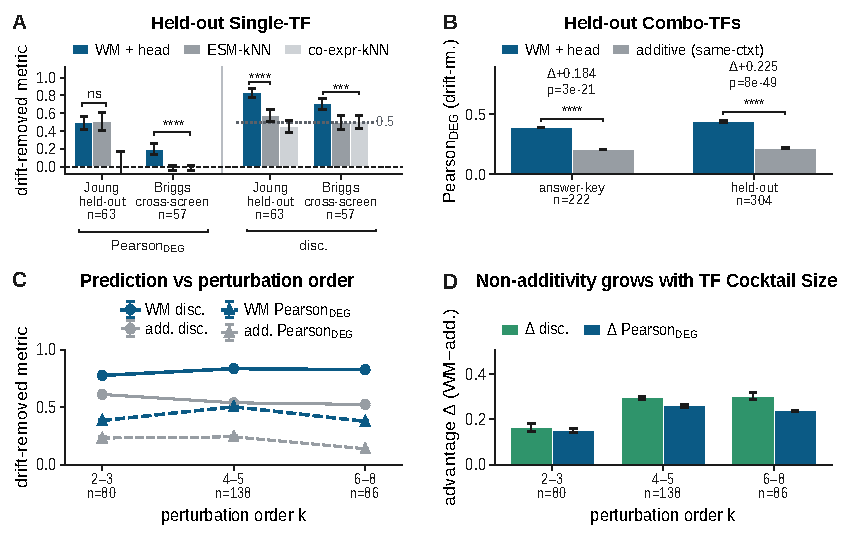
\includegraphics[width=0.92\linewidth]{figures/fig2.pdf}
\caption{\textbf{Held-out prediction beats a fair additive baseline.} (A) Single-TF prediction against ESM- and
co-expression-retrieval baselines (drift-removed \PearsonDEG and discrimination). (B) Held-out combinations
against the same-context additive baseline. (C) Metrics against perturbation order $k$. (D) The world-model
advantage grows with order. Mean over three seeds, SEM error bars, $n$ per panel.}\label{fig:pred}\end{figure}

\textbf{Setup and training.} We train the world model on two overexpression screens, the Joung single-TF atlas and the Briggs
combinatorial TF screen, over a shared $4366$-gene axis with $d{=}357$ GO:BP program latents, trained in two stages. First we fit a base model on single-TF perturbations, which learns one shift per TF. Then we
finetune this base on TF combinations, and we oversample the single-TF examples $8\times$ so the model keeps
its single-TF accuracy as it learns combinations. We build two checkpoints from this recipe. The deployable
checkpoint trains on all $495$ single-TF perturbations and all $1622$ combinations (arrayed Joung pairs and
pooled Briggs sets of up to eight TFs) and holds out only the $222$ Briggs HSPC-reaching validated combinations. However, for the held out predictions shown in Fig.~\ref{fig:pred}, we train a similar model with held out single and combination TFs with a  $85\%/80\%$ single/combination split across
three seeds, alongside sampled replays of earlier training data during finetuning to ensure model won't forget single-TF level prediction, and we report the held out values on this sibling model. For the downstream policy training, we
split fate targets by fate name into disjoint folds and always hold out the HSPC fate. Appendix~\ref{app:data}
gives the full data, splits, and hyperparameters along with methodological details.



\textbf{Evaluating the World Model} Overexpressing any TF at high MOI produces a large response that is largely shared across factors — a generic overexpression signature, pronounced here because many assayed TFs are master regulators. This shared component is a confound: a model that predicts it for every perturbation scores well on raw correlation while distinguishing no TF from any other, which is precisely the mechanism by which deep models tie simple baselines on published benchmarks  \citep{ahlmanneltze2025}. We therefore evaluate on the TF-specific residual. We estimate the drift as the mean single-TF $\Delta$ over the training set only, subtract it from both prediction and observation, and report two drift-removed quantities. $\mathrm{Pearson}_{\mathrm{DEG}}$ is the Pearson correlation between the drift-removed
predicted and observed change on the perturbation's differentially expressed (DE) genes (log-fold-change
above $0.1$, with the perturbed TF excluded), and measures whether the predicted response has the right
shape. Discrimination ($\mathrm{disc}$) is the area under the ROC of matching a prediction to its own
held-out perturbation against all others by drift-removed similarity, and measures whether the response
is specific to the right TF rather than a generic perturbation signature. We compare against a
same-context additive baseline that sums observed single-TF $\Delta$ vectors, a no-change baseline, and a
context-mean baseline \citep{ahlmanneltze2025}. For single-TF prediction we add two retrieval baselines
that copy the drift-removed response of the nearest training TF, by ESM2 similarity or by co-expression.

\textbf{Held-out single-TF prediction.} On held-out single TFs the world model is competitive with the
strongest baseline and far more specific (Fig.~\ref{fig:pred}A). On held-out Joung single TFs it
matches the ESM2 nearest-neighbour copy in $\mathrm{Pearson}_{\mathrm{DEG}}$ ($0.50$ against $0.51$) but
separates the perturbations much better in discrimination ($0.83$ against $0.58$), and on Briggs single-TF
effects, a cross-screen test to see whether model, that only saw Briggs combinations, can still generalize to singles, it outperforms every baseline on both
metrics for single TF perturbation prediction.


\textbf{The world model beats a fair additive baseline on combinations.} Now, testing the models performance on predicting combos of TFs given a cocktail set $S$, on held-out combinations, the
model beats the same-context additive baseline by $0.18$ to $0.23$ in $\mathrm{Pearson}_{\mathrm{DEG}}$,
a gain of $+0.184$ on the $222$ held-out answer-key combinations ($p{=}2.8\times10^{-21}$) and $+0.225$
on the $304$ held-out combinations ($p{=}8.4\times10^{-49}$) over three seeds (Fig.~\ref{fig:pred}B). The
advantage persists to high order. At $k{=}6$ to $8$ TFs the model reaches discrimination $0.84$ and
$\mathrm{Pearson}_{\mathrm{DEG}}$ $0.38$ against $0.53$ and $0.15$ for the additive baseline ($n{=}86$,
$p{=}3.1\times10^{-15}$), and it beats additive on $95\%$ of held-out combinations (Fig.~\ref{fig:pred}C,D),
so the non-additive margin grows with combination order.

\begin{figure}[t]\centering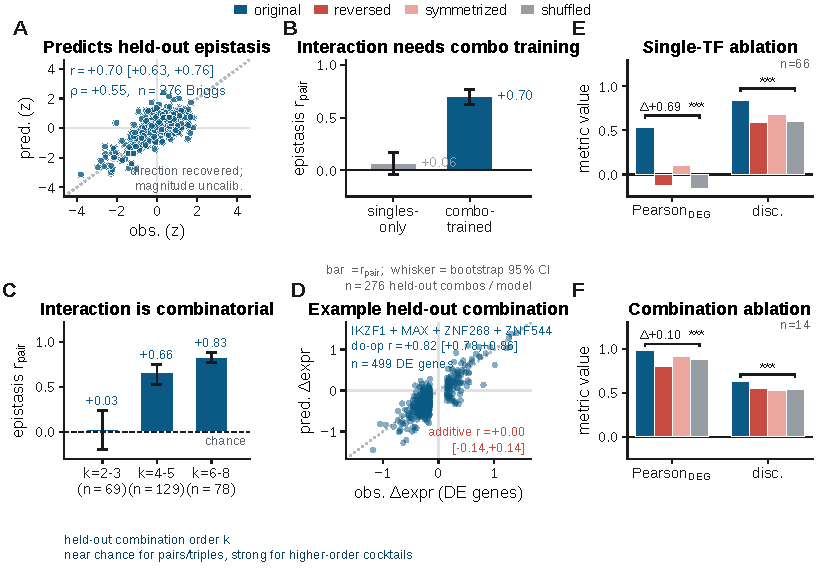
\includegraphics[width=0.92\linewidth]{figures/fig3.pdf}
\caption{\textbf{Combinatorial epistasis, and a load-bearing causal graph.} (A) Predicted against observed
interaction on $n{=}276$ held-out Briggs combinations ($r{=}0.70$). (B) A singles-only model captures none.
(C) Concordance rises with combination order. (D) An example held-out combination. (E, F) Single-TF and
combination prediction under original, reversed, symmetrized, and shuffled $A$, over $n{=}66$ held-out single
transcription factors and $n{=}14$ held-out combinations. Bars are point estimates tested against a
$1000$-shuffle-$A$ permutation null (stars) and a paired Wilcoxon over the held-out units ($p{=}9\times10^{-11}$
and $6\times10^{-5}$). Reversing the edges is as damaging as shuffling, so the dependence is directional
(drift-removed Pearson gaps of $0.69$ and $0.10$ over the null).}\label{fig:epi}
\end{figure}
% -- get p value for the bars
% -- LFC threshold on the DE genes
% -- subtext

\textbf{Epistasis is captured, and it comes from the interaction head.} We measure the interaction, or
net epistasis, as the combination response minus the sum of its single-TF responses. On held-out
combinations the model predicts the observed interaction at Pearson $r{=}0.70$ over $n{=}276$ Briggs
combinations (Fig.~\ref{fig:epi}A). The signal is concentrated in higher order. Broken out by order, the
held-out concordance is near chance for pairs and triples ($k{=}2$--$3$, $r{=}0.03$) and strong for
larger cocktails, reaching $r{=}0.66$ at $k{=}4$--$5$ and $r{=}0.83$ at $k{=}6$--$8$
(Fig.~\ref{fig:epi}C). This is exactly the part the model learns through the rank-$32$ interaction head
of \S\ref{sec:wm}. A singles-only model, whose head is never trained and stays zero, captures none of it
($r_{\mathrm{pair}}{=}0.06$), while the combination-trained model reaches $r_{\mathrm{pair}}{=}0.70$
(Fig.~\ref{fig:epi}B). The model recovers the sign and ranking of the interaction but not its magnitude,
which shows up as a sub-additive offset we report rather than hide.

\textbf{Is the causal graph load-bearing?}\label{sec:causal} Prediction accuracy alone does not tell us whether the
latent structural causal graph $A$ is actually \emph{used} for prediction, or whether it is an inert byproduct of
training. We test this by ablating $A$ inside the frozen do-operator and re-measuring prediction, and we then
characterize the biological structure of the learned graph.

\textbf{The directed graph is load-bearing for prediction} (Fig.~\ref{fig:epi}E). We ablate $A$ inside the
frozen do-operator by reversing, symmetrizing, or shuffling its edges, and re-measure
$\Delta$-prediction on the deployable model (a relative true-vs-shuffled comparison on the same
perturbations, so it does not need a held-out split). Against a 1000-shuffle null, single-TF prediction collapses from
Pearson $0.536\,[0.443,0.625]$ to a shuffled mean of $-0.156\pm0.010$, a gap of $0.692$ that no shuffle approaches (permutation $p<0.001$, $0/1000$, paired Wilcoxon across $66$ TFs
$p{=}8.9\times10^{-11}$, App.~\ref{app:causalsupp}), and $59$ of $66$ TFs individually
predict worse under a shuffled graph (App.~\ref{app:causalsupp}). Reversing the direction of edges is as damaging as shuffling
them, so the dependence is on edge \textit{direction}, not connectivity alone, the signature of the continuous do-operation and interventional training.  The same directional dependence holds on combinations, where all 14 held-out sets predict worse under a shuffled graph (gap $0.102$, permutation $p<0.001$,
Wilcoxon $p{=}6.1\times10^{-5}$). The effect is consistent across metrics as well. Reversing or shuffling $A$ collapses cross-fate discrimination
AUROC from $0.84$ to $0.60$ for single TFs (Fig.~\ref{fig:epi}E,F), and top-1 driver recall from $0.73$ to
$0.02$ (App.~\ref{app:causalsupp}).

\textbf{The latent graph is biologically structured.} The masked decoder pins each
latent axis to a named GO:BP program at mask coherence $1.00$, and the learned adjacency $A$ is a sparse signed
graph over those programs whose highest-connectivity hubs are developmental programs. Compared against known
biological priors (CollecTRI, DoRothEA, STRING), the projected graph carries above-chance signal but does not
beat a plain co-expression control, as expected for a context-specific model trained prior-off on TFs alone. We
therefore make no claim of literal GRN recovery and restrict the causal claim to prediction
(Sec.~\ref{sec:limits}).

\section{A goal-conditioned GFlowNet planner}\label{sec:planner}
\begin{figure}[t]\centering\panel{figures/fig4.pdf}{Fig planner: GFlowNet over frozen world model}
\caption{\textbf{Goal-conditioned GFlowNet planner.} A target fate conditions a trajectory-balance GFlowNet that
proposes a TF cocktail. The frozen do-operator propagates the injected shifts over the learned causal graph $A$ to
predict the $\Delta$ state, and the reward measures closeness to the target. The policy is trained by the
trajectory-balance gradient with a goal-conditioned $\log Z$ head.}\label{fig:planner_arch}\end{figure}

\textbf{Planning against the frozen causal world model.} Given a target fate we want to propose TF cocktails that
steer a control cell toward it, without re-running a search for every new fate. We train a goal-conditioned
policy that proposes a cocktail. The frozen do-operator of \S\ref{sec:wm} predicts the resulting $\Delta$ state
by propagating the injected shifts over the learned causal graph $A$, and the reward $\Phi(x,g)$ is the
drift-removed agreement of that predicted $\Delta$ with the target fate's observed signature
(Fig.~\ref{fig:planner_arch}). The causal graph is the planner's prior: through the do-operator it defines which
cocktails are predicted to reach which fates. At deployment the policy proposes candidates directly, with no
per-fate search.

\textbf{Why a GFlowNet, conditioned on the goal.} Many distinct TF sets can steer a cell to the same fate, so we
want a planner that \emph{samples} diverse cocktails in proportion to reward rather than collapsing onto a single
mode. We train a trajectory-balance GFlowNet \citep{bengio2021gflownet} whose partition-function head is
conditioned on the target fate, $\log Z(g)$. This goal-conditioning is what lets the policy spread its mass
across modes. A shared $\log Z$ head instead collapses onto the reward argmax (App.~\ref{app:rl}).

\textbf{An ensemble-pessimistic reward.} Because the world model is an imperfect oracle that a planner could
exploit, we score each cocktail under an ensemble of $K{=}6$ independently trained world models and reward the
pessimistic estimate $\Phi_{\mathrm{pess}} = \mathrm{mean}_k\,\Phi^{(k)} - \lambda\,\mathrm{std}_k\,\Phi^{(k)}$,
which penalizes cocktails the ensemble disagrees on. A modest $\lambda{=}0.25$ gave the best
recovery--diversity trade-off. The policy head is a plain per-slot multilayer perceptron over the shared
candidate vocabulary. Full training and hyperparameter details are in App.~\ref{app:hparams} and the complete
cross-arm evaluation in App.~\ref{app:rl}.

\FloatBarrier
\section{Cell-fate design results}\label{sec:rl}
\begin{figure}[t]\centering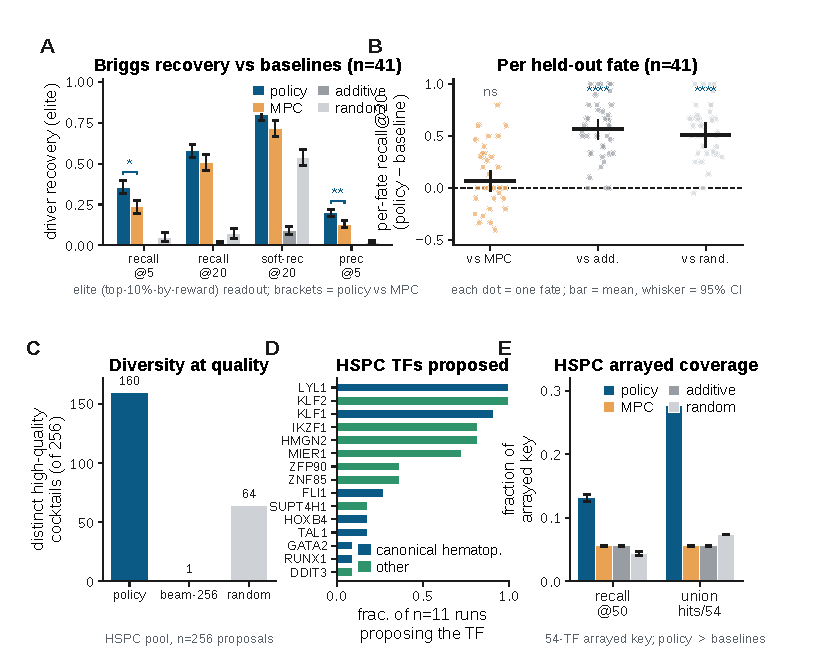
\includegraphics[width=0.86\linewidth]{figures/fig5.pdf}
\caption{\textbf{Cell-fate design: recovery, diversity, and zero-shot HSPC.} Recovery panels use the elite
(top-$10\%$-by-reward) readout on $n{=}41$ held-out Briggs fates, budget-matched to model-predictive control
(MPC), additive, and random baselines on the same fates. (A) Briggs recovery across four metrics (mean$\pm$SEM
over fates). (B) Per-fate elite recall@$20$, policy minus each baseline (one dot per fate): parity with MPC (ns),
far above additive and random ($p<10^{-4}$). (C) Distinct high-quality cocktails from $256$ HSPC-pool proposals.
(D) Arrayed-key TFs the policy proposes zero-shot on the held-out HSPC fate, bar is the fraction of $11$ runs
proposing each, colored canonical hematopoietic versus other. (E) Coverage of the $54$-TF Briggs arrayed key
($28$ combinations), elite recall@$50$ and distinct drivers surfaced, policy versus baselines.}\label{fig:rl}\end{figure}

\textbf{Protocol.} We evaluate the planner on four target-fate sources (Joung single- and combination-defined
fates, the Briggs hESC-to-HSPC screen, and a held-out zero-shot HSPC fate) under a leakage-clean fold-by-name
split over five seeds and three folds. The policy draws $N{=}256$ candidate cocktails per fate, read out by their
elite (top-decile by reward) frequency at no extra world-model cost. We compare against budget-matched baselines:
model-predictive control (MPC, beam search over the same shortlist, ${\approx}9{,}240$ world-model evaluations per
fate), a greedy beam-$1$ variant, an additive single-TF baseline, and random shortlists. Because the elite readout
is reward-guided, its chance level is a reward-matched null, and we test each method's gain over it with a paired
Wilcoxon across held-out fates. App.~\ref{app:metrics} defines every metric.

\textbf{Recovery matches exact search and dominates the heuristics, at a fraction of the compute}
(Fig.~\ref{fig:rl}A,B). On the $41$ held-out Briggs fates the policy beats the budget-matched additive and random
baselines on every metric by a wide margin (paired per-fate Wilcoxon $p<10^{-4}$ throughout), recovering $0.58$ of
the answer-key drivers at elite recall@$20$ against $0.01$ and $0.07$ for the additive and random baselines.
Against exact model-predictive control (MPC) beam search it is at parity on the broad metrics, elite recall@$20$
$0.58$ against $0.51$ and soft driver recall@$20$ $0.80$ against $0.72$ (paired Wilcoxon $p{=}0.1$ and $0.2$, not
significant, Fig.~\ref{fig:rl}B), and it is significantly \emph{ahead} at the top of the ranking, recall@$5$
$0.36$ against $0.24$ and precision@$5$ $0.20$ against $0.13$ (both $p<0.05$). It reaches this while drawing its
$256$ cocktails with ${\approx}36\times$ fewer world-model evaluations than beam search, an amortized single pass.
By source the recovery concentrates on Briggs, the two Joung sources sitting near the matched-null floor
(App.~\ref{app:rl}).

\textbf{Composition, not addition, is what the planner exploits.} The recovered cocktails are large, six to eight
transcription factors on the Briggs fates, and their predicted effect is strongly non-additive. This is the same
higher-order interaction the world model captures on held-out combinations, where concordance rises from near
chance for pairs to $r{=}0.83$ at order six to eight (Fig.~\ref{fig:epi}C), and it is exactly what an additive
single-TF baseline cannot represent, which is why that baseline sits at the null. The planner inherits this
combinatorial structure through the do-operator and uses it to assemble sets whose joint predicted effect exceeds
the sum of their single-TF parts.

\textbf{The policy is diverse at fixed quality, and search is not} (Fig.~\ref{fig:rl}C). For each held-out HSPC
fate we draw $256$ candidate cocktails from each method and set an arm-independent quality bar at the $75$th
percentile of the reward of matched-random cocktails, then count how many \emph{distinct} cocktails each method
proposes \emph{above} that bar, so the metric credits diversity only among high-reward designs and not a flood of
low-quality ones. The policy returns roughly $160$ such distinct high-quality cocktails, a random sampler $64$,
and beam search $1$, as beam is a single-solution optimizer rather than a sampler. Diversity at fixed quality, not
raw recovery, is where amortization is uniquely useful, handing an experimentalist many equally good candidates to
array rather than one.

\textbf{Zero-shot HSPC is a diversity-coverage advantage} (Fig.~\ref{fig:rl}D,E). We test the frozen policy
zero-shot on a held-out hESC-to-HSPC fate against the Briggs arrayed answer key ($54$ driver TFs across $28$
arrayed-validated combinations). On this broad key the policy's diverse elite proposals cover far more of
the answer key than search or the heuristic baselines, an arrayed recall@$50$ of $0.13$ against $\le0.06$ and
$15$ of the $54$ drivers surfaced across runs against $3$--$4$ for the baselines (Fig.~\ref{fig:rl}E). The
proposed factors are biologically coherent (Fig.~\ref{fig:rl}D): with the regulatory prior switched off the
policy nominates the canonical hematopoietic regulators LYL1, KLF1, KLF2, and IKZF1 in nearly every run, and
members of the blood stem-cell heptad \citep{wilson2010heptad}, TAL1/SCL, GATA2, RUNX1, and FLI1, together with
the stem-cell self-renewal factor HOXB4 \citep{antonchuk2002hoxb4}, in a minority of runs. This is a coverage
advantage of a diverse proposer over narrow search, not a per-driver precision result. On the narrow twelve-TF
named answer key the policy does not beat model-predictive control, and we do not calibrate a breadth-matched null
for the arrayed key, both of which we report rather than hide in App.~\ref{app:rl}.

\textbf{What the design choices buy} (App.~\ref{app:rl}). Goal-conditioning the partition function is what spreads
sampling across modes, as a shared partition function collapses onto the reward argmax and loses the diversity
above. The ensemble-pessimism weight $\lambda$ trades recovery against diversity, with $\lambda{=}0.25$ at the
knee, and the plain per-slot policy head matches heavier alternatives, so the amortization gain is not an artifact
of head capacity.

\textbf{Honest limits.} The cocktails point toward the target fate in world-model $\Delta$-direction
(own-minus-other cosine $+0.25$ on Briggs, $+0.19$ on HSPC) but do not discriminate fates by answer-key overlap, a
cross-fate discrimination wall (policy well below the driver oracle) we report rather than hide. The two Joung
sources are not significant, a training-data coverage limit rather than a method failure (Sec.~\ref{sec:limits}).

\textbf{Takeaway.} The planner is an amortized proposer rather than an oracle. On the well-powered Briggs source it
reaches the recovery of exact search at a small fraction of the world-model compute and returns two orders of
magnitude more distinct high-quality cocktails, and on a fully held-out HSPC fate its diverse proposals cover more
of the arrayed answer key with biologically coherent regulators than search does. The two Joung fate sources,
with only six and two held-out fates and one-to-five-TF answer keys, are underpowered and sit at the matched
null, and where fates share drivers the policy cannot yet separate them. We read these as evaluation and
discrimination frontiers for the next round of screens and models, not as evidence against amortized fate design.

\FloatBarrier
\section{Related work}\label{sec:related}
\textbf{Models of perturbation response.} Our world model descends from causal-disentanglement variational
autoencoders with soft interventions, including Discrepancy-VAE \citep{zhang2023discrepancyvae}, its
gene-ontology-structured variant SENA \citep{sena2025}, sparse additive mechanism-shift autoencoders
\citep{samsvae2023}, and Biolord \citep{biolord2024}, all of which amortize the response through an encoder pass.
We differ by treating the learned structural equation model as a frozen simulator whose multi-perturbation
response is an exact fixed-point solve (Eq.~\ref{eq:doop}), which is what makes zero-shot composition of unseen
cocktails well defined. This exact-by-design choice is motivated by audits showing that deep perturbation
predictors do not reliably beat simple additive or nearest-neighbor baselines on held-out perturbations
\citep{ahlmanneltze2025,perturbench2024}, and training with the regulatory prior off follows benchmarks showing
that context-independent priors can hurt context-specific inference \citep{genernib2025}.

\textbf{Planning and amortized diverse sampling.} Concurrent work couples goal-conditioned reinforcement learning
to a single-cell foundation model \citep{dirl2025}, recovers reprogramming protocols from fitted network dynamics
\citep{wytock2024}, or searches directly for reprogramming transcription factors \citep{tfcomb}. These optimize
against a learned predictor or search a model once per target. We instead sample cocktails in proportion to a
frozen structural-causal reward with a generative flow network \citep{bengio2021gflownet}, whose calibrated
diversity fits fate design because many transcription-factor sets reach the same fate. Goal-conditioning the
partition function lets one policy serve many fates, turning per-fate search into an amortized proposer.

\section{Limitations and conclusion}\label{sec:limits}
\textbf{Limitations.} The learned graph is load-bearing for prediction but is not a recovered gene-regulatory
network, so we restrict the causal claim to prediction and leave a rotational ambiguity in the adjacency $A$
unresolved (Sec.~\ref{sec:pred}). The captured epistasis is higher-order, near chance for pairs and strong only
for larger cocktails, and its magnitude is uncalibrated even where its sign and ranking are right. On planning,
the two Joung fate sources are not significant, but that evaluation is underpowered rather than a method failure,
with only six single-defined and two combination-defined held-out fates carrying one-to-five-TF answer keys, and
the world model is itself trained on the Joung data. A cross-fate discrimination wall also remains for fates
defined only by a coarse expression signature. We expect more held-out fates and richer fate representations to
resolve both.

\textbf{Conclusion.} A frozen structural causal world model gives exact, compositional, zero-shot
multi-perturbation predictions, and a goal-conditioned generative flow network planner over it designs cell-fate
cocktails that match exact search at a fraction of the compute, propose far more diverse cocktails, and on a
zero-shot HSPC fate cover more of the hematopoietic answer key with biologically coherent regulators than search
does. We report where the approach works and where it does not, so the result is usable rather than oversold.

\FloatBarrier
\bibliographystyle{plainnat}
\bibliography{references}

\appendix
% =============================================================================
%  EXPANDED APPENDIX  --  \input after \appendix in main.tex
%  No preamble, no \begin{document}. Sequence of \section blocks only.
%  Notation matches main.tex (z, A, S_g, u, D, Eq.~\ref{eq:doop}).
% =============================================================================

\section{Model and objective in full}\label{app:model_full}
This section gives the world model and its training objective at the level of exact
shapes and hyperparameters. All shapes below are those of the deployed world model at
epoch $60$. The gene axis has $G{=}4366$ genes and the latent has $d{=}357$ gene
programs. The decoder weight has shape $4366\times357$, the latent directed graph $A$ has
shape $357\times357$, and the per-TF label matrix has shape $4366\times100$.

\subsection{Encoder and latent variables}
The encoder is an amortized Gaussian. It reads a cell expression vector
$x\in\mathbb{R}^{4366}$ concatenated with a $16$-dimensional modality embedding
(Joung is modality $0$, Briggs is modality $1$) and maps the $4382$-dimensional input
through a hidden layer of width $512$ to a mean $\mu$ and log-variance
$\log\sigma^2$ over the exogenous term $\epsilon\in\mathbb{R}^{357}$. The first encoder
weight therefore has shape $512\times4382$ and the modality embedding table has shape
$2\times16$. We sample $\epsilon$ with the standard reparameterization. The
observational forward pass solves the latent structural equation model (SEM) for $z$
and decodes $x{=}Dz{+}b$.

\subsection{The latent SEM and its closed-form solve}
We model the resting latent state by a linear SEM over a learned signed directed graph
$A\in\mathbb{R}^{357\times357}$ driven by $\epsilon$,
\begin{equation}
z \;=\; A^{\top} z + \epsilon
\;\;\Longleftrightarrow\;\;
(I-A^{\top})\,z=\epsilon
\;\;\Longrightarrow\;\;
z=(I-A^{\top})^{-1}\epsilon .
\label{eq:sem_solve}
\end{equation}
The closed form follows because $I-A^{\top}$ is invertible whenever the spectral
radius of $A$ is below $1$. We enforce that by a power-iteration spectral-norm clamp
that rescales every sampled $A$ so $\lVert A\rVert_2 \le 0.85$, which guarantees
$I-A^{\top}$ is nonsingular and every downstream solve is well posed. The solve itself
is a direct linear solve with a sanitized escalating-ridge fallback for the rare
early-training singular case. The adjacency is a factored Gumbel-sigmoid gate times a
real-valued weight times a no-self-loop mask,
$A_{ij}=\mathrm{gate}_{ij}\cdot w_{ij}\cdot(1-\delta_{ij})$, with
$\mathrm{gate}_{ij}=\sigma((\theta_{ij}+\text{Gumbel})/\tau)$ in training and the hard
threshold $\mathbf{1}[\sigma(\theta_{ij}/\tau)>0.5]$ at evaluation. The temperature
$\tau$ anneals from $1.0$ to $0.25$ over training. At evaluation the graph is therefore
deterministic and signed.

\subsection{The shift-mutilate do-operator and $k$-TF composition}
A perturbation of a transcription factor (TF) $g$ enters as a soft intervention with two
parts. First it adds a program-space shift $S_g\in\mathbb{R}^{357}$. Second it applies a
per-program mutilation gate $u_g\in[0,1]^{357}$ that partially severs incoming edges. For
a set $\mathcal{P}$ of perturbed TFs the deployed operator sums the single-TF shifts,
injects the sum into the exogenous term, forms one aggregate gate, and does one mutilated
solve. This is Eq.~\eqref{eq:doop} of the main text. Concretely, in the structural
intervention mode used throughout,
\begin{align}
S &= \textstyle\sum_{g\in\mathcal{P}} S_g \;(+\,S_{\mathrm{int}}), &
\tilde{\epsilon} &= \epsilon_0 + S, \label{eq:doop_struct}\\
u &= \operatorname*{mean}_{g\in\mathcal{P}} \operatorname{clip}\!\big(\beta\lvert S_g\rvert,\,0,\,1\big),\ \beta{=}1, &
z_{\mathrm{post}} &= \big(I-\operatorname{diag}(1-u)A^{\top}\big)^{-1}\tilde{\epsilon}. \nonumber
\end{align}
Two design points matter. The gate $u$ is the per-single mean of $\operatorname{clip}(\beta\lvert S_g\rvert)$
rather than $\operatorname{clip}(\beta\lvert\sum_g S_g\rvert)$. The summed form saturates
about $41\%$ of programs to $u{=}1$ on combinations, which detaches $A$ and degrades
combination prediction, so we use the per-single mean, which is identical for a single TF.
In structural mode the shift is injected only into
$\tilde{\epsilon}$, so any non-target program moves only through $A$. If $A{=}0$ there is
no downstream effect, which is what makes $A$ load-bearing for prediction by construction.
The operator reduces to the additive shift $z_{\mathrm{prev}}+z_S$
when $u\to1$ on all driven programs and to predict-control when $u\to0$. Non-additivity
for combinations arises because $u$, and hence $M=\operatorname{diag}(1-u)$, depends
nonlinearly on the perturbed set. An optional symmetric low-rank interaction head adds a
combination-specific shift $S_{\mathrm{int}}=W_{\mathrm{out}}\big(\tfrac12((\sum_i x_i)^2-\sum_i x_i^2)\big)$
with $x_i=U(\text{ESM}_i)$ and an interaction rank of $32$. $S_{\mathrm{int}}$ is $0$ for a
single gene. The operator is validated against a naive fixed-point solve. A $k$-TF
prediction is therefore one linear solve assembled from
the same single-TF shifts used for singles, exact and zero-shot for novel combinations.

\subsection{Per-TF shift from ESM embeddings}
The shift $S_g$ is produced by a learned shift encoder from a per-gene descriptor
$\ell_g$. The descriptor is an ESM2 (Evolutionary Scale Modeling v2) protein language
model embedding of the TF, reduced by principal component analysis and z-scored to $100$
dimensions. The descriptor exists for
any TF in the panel, including held-out TFs, which is what lets the shift generalize
zero-shot. The encoder is a one-hidden-layer multilayer perceptron (MLP) of width $1024$
with a LeakyReLU$(0.2)$ nonlinearity mapping $100\to357$, with a raw real-valued output and
no output activation. Its first weight has shape $1024\times100$ and its output weight has
shape $357\times1024$. A second head shares the trunk and emits per-program
gate logits, so the shift is $S_g=c\cdot(\text{gate}\odot\text{raw})$ with a learned scalar
penetrance $c$ and a sparse target gate that is Gumbel-sigmoid in
training and hard at evaluation. The gate open
probability is penalized by an $L_0$ target-sparsity term. A leakage-safe train-only
retrieval memory over embedding keys can add an embedding-similarity-weighted shift with
the query row self-masked, which we keep off by default in the reported model.

\subsection{The masked gene-program (SENA) decoder}
The decoder is linear, $x{=}Dz{+}b$ with $D\in\mathbb{R}^{4366\times357}$. Each latent
column is tied to a Gene Ontology Biological Process (GO:BP) program by a membership mask
$M\in\mathbb{R}^{4366\times357}$. We refer to this masked gene-program decoder scheme as
SENA, following \citep{sena2025}. The effective decoder weight is the masked-learnable
product $D\odot M$, so annotated gene-program pairs learn at full strength while
off-annotation pairs are shrunk by a leak factor $\lambda$. This forces gene covariance to
route through the program latents and $A$ rather than through arbitrary gene-gene edges.
The mask is built from the Enrichr GO Biological Process 2023 library. Candidate terms are
GO:BP sets with at most $30$ genes and at least $5$ genes present on our axis. Terms are
greedily de-duplicated largest-first so no kept term overlaps a previously kept one by more
than $0.5$ under the containment overlap
$\lvert A\cap B\rvert/\min(\lvert A\rvert,\lvert B\rvert)$. Off-annotation entries take the
leak value $\lambda{=}0.3$. The GO:BP selection yields $357$ kept programs on our axis, so
the latent dimension is set to the number of kept programs and the deployed model has
$d{=}357$ program latents. The decoder mask is not frozen, so $D$ is masked-learnable
rather than fixed to the mask.

\subsection{Training objective, prior-off}
The total loss is
\begin{equation}
\begin{split}
\mathcal{L}
={}& \lambda_{\mathrm{rec}}\,\mathcal{L}_{\mathrm{rec}}
+ \beta_{\mathrm{eff}}\,\mathcal{L}_{\mathrm{KL}}
+ \lambda_{\mathrm{pert}}\,\mathcal{L}_{\mathrm{pert}}
+ \lambda_{\mathrm{spec}}\,\mathcal{L}_{\mathrm{spec}}\\
&+ \lambda_{\mathrm{ortho}}\,\mathcal{L}_{\mathrm{ortho}}
+ \lambda_{\mathrm{sparse}}\,\mathcal{L}_{\mathrm{sparse}}
+ \lambda_{\mathrm{prior}}\,\mathcal{L}_{\mathrm{prior}} .
\end{split}
\label{eq:total_loss}
\end{equation}
We train prior-off. The graph prior, decoder-orthogonality, graph-sparsity, decoder-$L_1$,
and acyclicity weights are all zero
($\lambda_{\mathrm{prior}}{=}0$, $\lambda_{\mathrm{ortho}}{=}0$, $\lambda_{\mathrm{sparse}}{=}0$,
$\lambda_{\mathrm{D\text{-}sparse}}{=}0$, and both acyclicity coefficients $0$),
so no external transcription-factor--target database edge is ever used to shape $A$. The
acyclicity term is skipped entirely when its weights are zero to avoid $0\times\text{NaN}$
poisoning. The training log confirms the acyclicity residual stays at $0$ throughout.
Table~\ref{tab:loss_terms} lists every active term with its exact form and weight for the
deployed model.

The reconstruction term is a plain mean squared error (MSE), modality-gene-masked so a
cell only scores genes its modality observes. The Kullback--Leibler (KL) divergence is the
standard diagonal-Gaussian variational term with a free-bits floor, and its weight $\beta$
ramps linearly from $0.01$ to $0.5$ over the first $30$ epochs. The perturbation term
$\mathcal{L}_{\mathrm{pert}}$ (weight $\lambda_{\mathrm{pert}}{=}10$, clamped at $50$ before
scaling) is the sum of the sub-terms in Table~\ref{tab:loss_terms}, computed on cell
sentences of $S{=}64$ cells so the mean-shift target is a per-sentence pseudobulk $\Delta$.
The DE-gene MSE sub-term deliberately preserves magnitude and is not whitened, and is
restricted to observed differentially expressed (DE) genes above the threshold $0.1$, which
is the term that carries per-gene response magnitude.

\begin{table}[h]\centering\footnotesize
\caption{Active training-loss terms for the deployed world model. All weights are exact
configured values. Terms with weight $0$ are omitted (graph prior, decoder-orthogonality,
graph-sparsity, decoder-$L_1$, acyclicity, energy optimal-transport, and shift-$L_1$).
MMD denotes maximum mean discrepancy and InfoNCE the info-noise-contrastive estimation
loss.}
\label{tab:loss_terms}
\begin{tabular}{@{}llll@{}}
\toprule
Term & Form (drift $=$ mean train-single $\Delta$) & Weight & Value \\
\midrule
Reconstruction & $\lVert (\hat{x}-x)\odot m_{\mathrm{mod}}\rVert^2$ mean-MSE & $\lambda_{\mathrm{rec}}$ & $1.0$ \\
KL & $-\tfrac12\overline{(1+\log\sigma^2-\mu^2-\sigma^2)}$, free-bits & $\beta$ & $0.01\!\to\!0.5$ \\
Perturbation MSE & $\lVert \Delta_{\mathrm{pred}}-\Delta_{\mathrm{obs}}\rVert^2$ & $\lambda_{\mathrm{MSE}}$ & $1.0$ \\
Distribution matching (MMD) & Gaussian-RBF MMD$^2$, median bandwidth, per sentence & $\lambda_{\mathrm{MMD}}$ & $1.0$ \\
Goal specificity (InfoNCE) & symmetric NCE on drift-removed norm.\ $\Delta$, temp $0.2$ & $\lambda_{\mathrm{NCE}}$ & $1.0$ \\
DE-gene MSE & unwhitened MSE on $\{|\Delta_{\mathrm{obs}}{-}\mathrm{drift}|{>}0.1\}$ genes & $\lambda_{\mathrm{DEG}}$ & $8.0$ \\
Target sparsity ($L_0$) & $\overline{\sum_k \text{gate-prob}_k}$, ramped & $\lambda_{L_0}$ & $0.03$ \\
Spectral & $\operatorname{relu}(\sigma_{\max}(A)-0.95)$ & $\lambda_{\mathrm{spec}}$ & $0.1$ \\
\bottomrule
\end{tabular}
\end{table}

A gradient-reversal dataset classifier on the encoder mean $\mu$ drives latent
modality-invariance and is added with an implicit coefficient of $1.0$ when there is more
than one modality. The mutilation is run in shift mode with $\beta{=}1.0$. The mutilation
clip of $0.5$ is inert in shift mode, where the clamp is to $1.0$.

% =============================================================================
\section{Datasets, splits, and checkpoint discipline}\label{app:data}
\subsection{Sources}
We use three single-cell resources. The Joung TF atlas is a human embryonic stem cell
(hESC) single-TF overexpression atlas at day $7$ \citep{joung2023tfatlas}. It contributes
single-TF perturbations plus a small number of arrayed combinations. The Briggs
hESC$\to$fate overexpression screen is a dense combinatorial TF screen read out at days
$14$ and $28$, deposited at GEO under accession GSE328457 \citep{briggs2026}. It
contributes high-order TF combinations and pluripotent hESC-start controls. The Cao fetal
cell atlas defines the target-fate marker signatures \citep{cao2020fetal}.

\subsection{Gene axis and modality alignment}
The shared gene axis is the Joung $4366$-gene vocabulary. Briggs cells are aligned onto it
by matching counts-per-$10{,}000$ log-normalized values on shared genes and zero-filling
the rest. About $2800$ of the $4366$ genes are observed in Briggs. A per-modality gene mask
keeps the vocabulary at $4366$ but scores the reconstruction loss only on genes each
modality observes. Joung sees all $4366$ genes, Briggs only its observed subset. Each
Briggs cell carries an in-vocabulary TF set obtained by collapsing isoforms and keeping the
modelable TFs. Cells are grouped by their in-vocabulary TF set. Sets of in-vocabulary size
$2$ to $8$ with at least $5$ replicate cells become combination
perturbations. The per-cell median in-vocabulary set size is about $5$ and reaches into the
teens, so Briggs supplies the high-order regime.

\subsection{Answer-key holdout and leakage-free splits}
The answer key is held out of training so recovery is honest. A Briggs combination is held
out if it shares at least two members with $P_1$ or $P_2$, is one of the six canonical hematopoietic stem and progenitor cell (HSPC)
pairs, or is one of the arrayed-validated combinations from the supplementary table. The
two validated cocktails are
$P_1=\{\text{TAL1, RPA3, ZFP90, RNF138, LMO2, KLF2}\}$ and
$P_2=\{\text{DDIT3, MZF1, HOXB3, MIER1, SIRT6, ZNF85}\}$. In the deployed
model this holds $222$ answer-key combinations out of training while keeping them for
evaluation. Single TFs are
split with combo-involved TFs forced into training, so a single-TF holdout never silently
guts combination coverage.
Fate targets are split by fate name into folds to prevent cross-source leakage.

\subsection{The two deployed checkpoints}
Two checkpoints back the paper, both trained for $60$ epochs.

\textbf{Deployed production world model.} Trained with both the single-TF and combination
training fractions set to $1.0$, so every single TF and every non-answer-key combination is
in training and only the $222$ answer-key combinations are held out. Like the held-out
sibling, it warm-starts from a singles-only base model and oversamples single-TF sentences
$8\times$ during the combination finetune, so single-TF effects are retained. The training
log records $963{,}974$ cells, a per-epoch reconstruction subsample of $150{,}000$ cells,
$495$ single-TF blocks and $1622$ combination blocks ($2117$ blocks total), and $22{,}328$
cell sentences per epoch. This is the checkpoint used for all causal-structure validation
(App.~\ref{app:model_full} numbers and Sec.~\ref{sec:causal}) and as the frozen reward
oracle for the planner. Because its training fractions are $1.0$, a held-out-singles score
on this checkpoint measures memorization and is not a genuine held-out number. Genuine
held-out single and combination prediction uses the next checkpoint.

\textbf{Held-out combination finetune.} Trained with a single-TF training fraction of
$0.85$ and a combination training fraction of $0.8$ under a fixed split seed, warm-started
from a singles-only base model, with recency-weighted replay of combinations during the
finetune. This split yields $432$ train and $63$ held-out Joung singles, $36$ train and $8$
held-out Joung combinations, and Briggs combinations split into train and held-out plus the
$222$ answer-key combinations. Two additional seed variants provide the three seeds behind
the main-text prediction $p$-values. The main-text held-out advantages of $+0.184$
(answer-key combinations) and $+0.225$ (held-out combinations) in drift-removed
\PearsonDEG are computed on this checkpoint across the three seeds. The epistasis
panels (Fig.~\ref{fig:epi}A--D) also use this held-out sibling for the combination-trained
model and its singles-only base for the singles-only arm, so the interaction claims are
evaluated on the same recipe as the planner world model. Only the enrichment panel
(Fig.~\ref{fig:epi}E) uses the deployed production world model.

\subsection{Fate-target annotation}\label{app:fate}
Target fates are defined by a marker-signature pipeline over the Cao fetal cell atlas. We
start from the Cao cell-type mean log-expression profiles, restrict to genes on our shared
axis, and center them. Cell types are merged into fate groups by average-linkage
hierarchical clustering at cosine similarity $0.78$ on the centered profiles, and each fate
group is named by its dominant tissue--type suffix. For each fate group we take the top
$50$ genes by one-vs-rest over-expression as its marker set and form a normalized marker
signature.

Every candidate perturbation (Briggs combinations, Joung single-TF overexpressions, and
Joung arrayed combinations) is summarized by its drift-removed mean response, the residual
centroid $\Delta$ obtained by subtracting the source-level mean $\Delta$. Each perturbation's
residual $\Delta$ is scored against all marker signatures and assigned to its argmax fate. A
fate is \emph{kept} only if it is \emph{target-separable}, meaning its marker signature is
isolated from every other signature (max cosine similarity below $0.75$), and
\emph{reachable}, meaning it collects at least a minimum number of marker-argmax member
cells ($5$ for Briggs, $3$ for Joung). Each kept fate's target is the drift-removed mean
$\Delta$ (residual centroid) of its marker-argmax member cells. Kept fates are then tiered.
Tier~A fates additionally have a positive per-fate cosine silhouette in the marker-gene
(specific-gene) subspace, and Tier~B fates have a non-positive silhouette. Crucially, the
annotation does \emph{not} gate on silhouette. Both tiers are retained, and the silhouette
only labels the clean-answer-key core (Tier~A) versus the remainder (Tier~B). Reachable-fate
confidence uses a proper Benjamini--Hochberg correction, which moves the fate set by only one
or two Briggs fates relative to a raw permutation cutoff.

Each fate additionally stores its Cao marker genes, its member count, its driver TFs, and its
answer-key combinations. The driver and answer-key lists derive from the Briggs $P_1$/$P_2$
canonical cocktails and the arrayed-combo table (Sec.~\ref{app:data}). The pipeline yields
$84$ fates, namely $65$ Briggs, $16$ Joung single-TF, and $3$ Joung combination fates
(Table~\ref{tab:fates}). The zero-shot HSPC fate,
the Briggs liver hematopoietic-stem-cell fate (Tier~B), is forced to fold $-1$ and is always
held out. Its evaluation uses the dedicated Briggs $P_1\cup P_2$ answer key rather than Cao
markers.

Fates are split into a five-fold leave-fates-out cross-validation partition by \emph{fate
name}, so all sources of one fate name share a fold and there is no cross-source leakage. The
folds are stratified by name-level tier and assigned round-robin by descending member count,
so each Tier~A fate is held out exactly once. In each cross-validation fold $f\in\{0,\dots,4\}$
the fates assigned to fold $f$ are held out for evaluation and the rest are used for
training, and the single fate at fold $-1$ (HSPC) is held out in every fold. The per-fold
held-out counts are $19$, $18$, $14$, $16$, $16$ for folds $0$--$4$ plus the $1$ always-held-out
HSPC fate at fold $-1$.

\begin{table}[h]\centering\footnotesize
\caption{Fate-target counts by source and tier. Tier~A fates additionally clear a positive
marker-subspace silhouette (clean answer-key core). Tier~B fates are target-separable and
reachable but silhouette-negative. The HSPC fate (the Briggs liver hematopoietic-stem-cell
fate) is one of the $65$ Briggs fates, is Tier~B, and is forced to fold $-1$ (always held
out).}
\label{tab:fates}
\begin{tabular}{@{}lrrr@{}}
\toprule
Source & Fates & Tier A & Tier B \\
\midrule
Briggs (combinations)      & $65$ & $10$ & $55$ \\
Joung single-TF            & $16$ & $2$  & $14$ \\
Joung combination          & $3$  & $2$  & $1$  \\
\midrule
Total                      & $84$ & $14$ & $70$ \\
\bottomrule
\end{tabular}
\end{table}

% =============================================================================
\section{Training and planner hyperparameters}\label{app:hparams}
\subsection{World-model hyperparameters}
Table~\ref{tab:wm_hparams} lists the exact world-model settings for the deployed model.
Training runs in three phases inside the $60$ epochs, recorded in the training log. Phase A
is epochs $1$ to $10$, reconstruction only with the directed graph frozen. Phase B is epochs
$11$ to $50$, directed-graph learning active with the full loss. Phase C is epochs $51$ to
$60$, full loss with temperature annealing. The world model trains on CPU high-memory nodes
with about $340$ GB of RAM.

The architecture is the model of App.~\ref{app:model_full}: a per-cell encoder, a latent
SEM over $d{=}357$ GO:BP program latents solved in closed form, an ESM2 per-TF shift encoder
($100$-dim descriptor $\to$ $1024$ hidden $\to$ $357$), the shift-mutilate do-operator for
$k$-TF composition, and the masked-GO (SENA) linear decoder to the $4366$-gene axis. These
same settings train both deployed checkpoints described in Sec.~\ref{app:data} (``The two
deployed checkpoints''). The deployed production world model is the epoch-$60$ checkpoint,
used for all causal-structure validation and as the frozen planner reward oracle. The
held-out combination finetune shares every model hyperparameter in
Table~\ref{tab:wm_hparams} and differs only in its train fractions (single-TF fraction
$0.85$, combination fraction $0.8$) and its singles-only-base warm-start. It backs the
held-out prediction and epistasis panels. Both checkpoints warm-start from a singles-only
base and oversample single-TF sentences $8\times$ during the combination finetune.

\begin{table}[h]\centering\footnotesize
\caption{World-model hyperparameters for the deployed model. Values not present in the
configuration are marked not specified.}
\label{tab:wm_hparams}
\begin{tabular}{@{}llll@{}}
\toprule
Optimizer & Adam & Gene axis $G$ & $4366$ \\
Learning rate & $10^{-3}$ & Latent programs $d$ & $357$ (GO:BP mask) \\
LR warmup epochs & $5$ & Decoder & masked-GO (SENA), $\lambda{=}0.3$ \\
Epochs & $60$ & Shift descriptor & ESM2, $100$-dim \\
Batch size & $256$ & Shift MLP & $100\!\to\!1024\!\to\!357$, LeakyReLU$(0.2)$ \\
Grad accumulation & $4$ & Interaction rank & $32$ \\
KL $\beta$ & $0.01\!\to\!0.5$ over $30$ ep & Graph samples (train/eval) & $1$ / $32$ \\
$\lambda_{\mathrm{pert}}$ & $10$ & Mutilation $u_{\max}$, $\beta$ & $0.5$, $1.0$ \\
DEG-MSE weight, thr & $8.0$, $0.1$ & Spectral weight & $0.1$ \\
Contrastive temp & $0.2$ & Prior / sparse / ortho / acyclicity & $0$ (prior-off) \\
Cell-sentence $S$ & $64$ & Sentences per block & $4$ \\
Sentence batch & $32$ & Single-sentence mult & $8$ \\
Recon subsample & $150{,}000$/epoch & $\tau$ anneal & $1.0\!\to\!0.25$ \\
\bottomrule
\end{tabular}
\end{table}

\subsection{The GFlowNet planner}
The deployed planner is a trajectory-balance generative flow network (GFlowNet) over the frozen world model. A cocktail
is built one TF at a time by an autoregressive forward policy. Because the construction is
autoregressive there is a single parent per state, so the backward policy is trivially
$P_B\equiv1$ and the trajectory-balance loss for a terminal cocktail $x$ under goal $g$ is
\begin{equation}
\mathcal{L}_{\mathrm{TB}}
=\Big(\log Z(g) + \textstyle\sum_t \log P_F(a_t\mid s_t,g) - \beta\cdot\Phi(x,g)\Big)^2 ,
\label{eq:tb}
\end{equation}
with reward $R(x)=\exp(\beta\,\Phi(x,g))$ \citep{bengio2021gflownet} and reward exponent
$\beta{=}48$. The deployed flagship uses a \emph{goal-conditioned} partition function
$\log Z(g)$, where a per-goal head absorbs the goal-dependent normalizer so the forward policy is
free to spread mass across the many high-reward cocktails for each goal. This is the single
most important lever for diversity. The alternative of a single shared scalar $\log Z$ for
all goals forces the forward policy to carry the goal-dependent normalizer, and it collapses
to an amortized argmax at convergence (effective number of distinct sampled sets
$\mathrm{ess}_q\approx1$--$2$, versus up to the target ceiling of $\approx46$ under the
conditional head). We report the shared-$\log Z$ variant as an ablation.

\paragraph{Ensemble-pessimistic reward.} The potential $\Phi(x,g)$ is the drift-removed match
of the world-model-predicted state to the target fate. To guard against exploiting any single
world model's errors, the reward is \emph{ensemble-pessimistic}. We evaluate the same cocktail
under $K{=}6$ independently trained world models and combine their potentials as
\begin{equation}
\Phi_{\mathrm{pess}}(x,g)=\operatorname*{mean}_{k=1}^{K}\Phi^{(k)}(x,g)\;-\;\lambda\cdot\operatorname*{std}_{k=1}^{K}\Phi^{(k)}(x,g),
\qquad \lambda=0.25 ,
\label{eq:pess}
\end{equation}
so cocktails on which the ensemble disagrees are penalized. The pessimism weight $\lambda$
trades recovery against sampling diversity. The deployed value is $\lambda{=}0.25$.

Off-policy replay mixes a fraction $\gamma{=}0.5$ of each batch from a recency-weighted buffer
of past cocktails (capacity $5000$), which is valid for trajectory balance. The reward oracle
is the frozen world-model ensemble, so no surrogate or acquisition proxy is needed. Batches
are $16$ trajectories per update, trained for $10^{6}$ iterations. The per-source action
budget is set at reset, so Joung caps at $k{\le}2$ and Briggs at $k{\le}8$. Prioritized,
reward-weighted replay is a reported negative (App.~\ref{app:rl}). The deployed setting is
plain recency-weighted replay.

The policy is a set-based autoregressive policy over the vocabulary
$\{\text{STOP}\}\cup\text{candidates}$. A shared encoder feeds all slots, so cost grows
linearly in $k$ not combinatorially. STOP is forbidden at slot $0$ and already-chosen genes
are masked at later slots. The action head is a plain multilayer perceptron (MLP)
over the per-slot features.

\subsection{Design selection}
The deployed flagship, the goal-conditioned GFlowNet with the plain MLP head and
$\lambda{=}0.25$, was selected by a sweep over the partition function (shared versus
goal-conditioned $\log Z$) and the ensemble-pessimism weight
$\lambda\in\{0.1,0.25,0.5,0.75,1.0\}$, at $10^6$ iterations across five folds and three seeds
on the frozen production world model with a curated candidate pool and per-source $k$ caps.
The goal-conditioned $\log Z$ is what enables diverse sampling and $\lambda{=}0.25$ gives the
best recovery--diversity trade-off (App.~\ref{app:rl}). The InfoNCE fate-specificity term uses
scale $\beta_{\mathrm{contrast}}{=}0.3$; a no-contrast control that drops it is reported in
App.~\ref{app:rl}.

% =============================================================================
\section{Evaluation metrics}\label{app:metrics}
This section defines every metric precisely. For a planner the per-fate output is a
frequency dictionary of proposed TFs over the best-of-$N$ samples. Picks are ranked by
descending selection frequency.

\textbf{Driver recall at $k$.} With driver set (answer key) $\mathcal{D}$ and the top-$k$
ranked picks $\mathcal{T}_k$, $\mathrm{drv\_recall}@k = \lvert\mathcal{T}_k\cap\mathcal{D}\rvert/\lvert\mathcal{D}\rvert$.
The denominator is the answer-key size, so this is recall not precision. We report
$k\in\{5,10,20\}$.

\textbf{Precision at $k$.} $\mathrm{prec}@k = \lvert\mathcal{T}_k\cap\mathcal{D}\rvert/\min(k,\lvert\mathcal{T}_k\rvert)$.
We report $k\in\{5,10\}$.

\textbf{Cross-fate discrimination, own minus other.} For a scorer $s$, discrimination is the
score of a fate's picks against its own answer key minus the mean score of the same picks
against every other held-out fate's answer key, $\mathrm{disc}=s(\text{own})-\overline{s(\text{other})}$.
We report $\mathrm{disc\_dr20}$ using recall@$20$ and
$\mathrm{disc\_soft1}$ using SOFT-1. The oracle plays the true drivers as picks. For
$\mathrm{disc\_dr20}$ the oracle equals $1-\overline{\text{cross-fate driver-set overlap}}$,
so a high oracle means the answer-key driver sets are nearly disjoint across
fates and a perfect selector separates them, while a low oracle means fates share drivers
and cap what any planner can achieve. A random planner sits near zero because its picks hit
own and other drivers equally.

\textbf{SOFT-1 and SOFT-2.} These score in a functional space built from drift-removed,
unit-normed single-TF $\Delta$ vectors with $k$-means module labels. SOFT-1 is the
frequency-weighted mean, over picks, of
the maximum cosine of a pick's single-TF $\Delta$ to any driver's single-TF $\Delta$. SOFT-2
is the frequency-weighted fraction of picks whose $k$-means module coincides with any driver's
module. The variants m12, m24, m48 use $12$, $24$, or $48$ modules. These metrics saturate.
The nearest-cosine over a broad answer set in a low-dimensional unit-normed space means even
random TFs land close to some driver and share one of only twelve modules, so a matched-random
null already scores about $0.28$ to $0.36$ and the policy barely separates. For this reason
SOFT-1 and SOFT-2 are reported in the appendix with their null values shown, and the
headline uses driver recall, precision, and the own-minus-other discrimination forms.

\textbf{Best residual match.} For each sampled cocktail the world model applies the
do-operator, decodes, subtracts the control reconstruction and the drift, and matches the
drift-removed predicted $\Delta$ against the target on the active dimensions. The best
residual match is the maximum match over the best-of-$N$ sampled cocktails.

\textbf{The matched-random null.} For each held-out fate the null records the policy's
per-sample cocktail sizes, then draws for each sample a random cocktail of the same size
from the candidate pool and recomputes every metric. The reported null value is the mean
over $R$ permutations ($R{=}500$ for the reported runs). When a policy is gated to a
per-goal shortlist, the reported evaluation draws the null from the full $280$-candidate
pool, which gives a pipeline-versus-ungated contrast consistent across all sources.

\textbf{The $1000$-shuffle-$A$ permutation test.} For the causal-structure claim we ablate
$A$ inside the frozen do-operator. The variants are original, reversed ($A^{\top}$),
symmetrized ($\tfrac12(A+A^{\top})$), and shuffled (a permutation of the off-diagonal
entries, which preserves the value multiset and edge count). Every non-original variant is
rescaled to
match $\lVert A\rVert_2$, so magnitude is not a confound. The null draws $N{=}1000$ shuffled
$A$ matrices, each with a fresh seed, and stores the mean drift-removed \PearsonDEG
across perturbations. The single-TF prediction metric is the per-perturbation Pearson of the
drift-removed predicted residual against the drift-removed observed residual on the set of
DE genes above the threshold $0.05$, with the perturbed TF itself excluded so the metric
measures downstream recovery. The permutation $p$-value is the add-one estimate
$(1+\#\{\text{null}\ge\text{original}\})/(N+1)$, which gives $1/1001\approx9.99\times10^{-4}$
when no shuffle exceeds the original.

\textbf{Paired Wilcoxon across fates and Benjamini--Hochberg.} The primary planner
significance test is a one-sided paired Wilcoxon signed-rank of the policy against its
matched-random null across held-out fates. The replicate is the fate when at least two
held-out fates exist, with per-fate values
averaged over seeds. For a single-fate source such as HSPC the test falls back to pairing
across the fold-by-seed training replicates, which gives up to $15$ paired points for five
folds and three seeds. Benjamini--Hochberg correction is applied across the whole
source-by-metric grid. The same one-sided paired Wilcoxon signed-rank test (dropping zero
differences) is used for the $66$-TF and $14$-combination causal-structure tests.

\textbf{Standard error of the mean (with one delta-degree-of-freedom).} Standard errors of the
mean, abbreviated s.e.m. in the tables and distinct from the structural equation model above,
use the per-seed means as the replicate axis. Within each seed, per-fate values are pooled
across folds and averaged, and the standard error of the mean is the sample standard
deviation of those per-seed means with one delta-degree-of-freedom
divided by $\sqrt{n_{\mathrm{seeds}}}$. A single replicate is reported as undefined rather
than zero.

\textbf{Baselines.} MPC-exact is a model-predictive control (MPC) world-model beam search (beam width $8$) that
forward-selects the cocktail maximizing the predicted drift-removed match. Additive-greedy
is a forward selection that sums observed drift-removed single-TF $\Delta$ vectors with no
world-model interaction. Random-shortlist is a single
random pick from the goal shortlist. Every baseline is restricted to the same per-goal
shortlist as the policy, so the comparison isolates selection within the pool.

% =============================================================================
\section{Full cross-arm planner evaluation}\label{app:rl}
The deployed planner is the goal-conditioned GFlowNet with the plain MLP head and the
ensemble-pessimistic reward at $\lambda{=}0.25$ (Eq.~\eqref{eq:pess}), trained over three
folds and five seeds. We evaluate it on two axes against non-learned baselines, asking (1) whether it
\emph{recovers} the true driver TFs of a held-out fate, and (2) whether it \emph{samples
diverse, reward-proportional} cocktails, with a zero-shot HSPC case study. The genuine wins
are that the planner is amortized and cheap, is diverse-at-quality, and on the zero-shot HSPC fate
covers more of the arrayed answer key with biologically coherent regulators than search does. On
per-driver recovery it reaches \emph{parity} with model-predictive beam search, not a win.

\paragraph{Why a GFlowNet trainer.} Against a one-step set-PPO trainer, the GFlowNet samples
many distinct high-quality cocktails while set-PPO collapses toward a single mode, which is
why the deployed planner is a GFlowNet rather than a policy-gradient trainer.

\subsection{Axis 1, driver recovery}
On the finalized flagship we report held-out Briggs recovery under three readouts of the
$256$ sampled cocktails, each against its \emph{matched} null (Table~\ref{tab:flagship_rec}).
The \emph{raw} readout ranks TFs by sampling frequency and is compared to a matched-breadth
permutation null ($\approx0.072$) that draws random size-matched cocktails and ranks them the
same way. The \emph{elite-$10$} readout keeps the top $10\%$ of the $256$ by reward and ranks
within that set, and the \emph{leave-one-out} (LOO) readout ranks each TF by its marginal
reward contribution. Both are compared to the \emph{random-plus-elite} null ($\approx0.42$),
which passes random cocktails through the same reward filter and so measures what the reward
filter alone buys. Using the weak permutation null on an elite readout would over-credit the
policy for the filter's work, so each readout is matched to its own null. Model-predictive
beam search is likewise a reward-guided selector, so the fair comparison between the policy
and beam search uses the common random-plus-elite null.

\begin{table}[h]\centering\footnotesize
\caption{Deployed flagship (goal-conditioned GFlowNet, MLP head, ensemble pessimism
$\lambda{=}0.25$), held-out Briggs driver recall at $20$, three folds $\times$ five seeds.
Each readout is scored against its matched null. Here $\Delta$ is the policy minus that null.
World-model (WM) evaluations per fate index inference cost. The random-plus-elite null is the
common reward-guided baseline used to compare the policy against beam search.}
\label{tab:flagship_rec}
\begin{tabular}{@{}llccc@{}}
\toprule
Planner / readout & null & abs r@$20$ & $\Delta$ vs null & WM evals/fate \\
\midrule
policy, raw            & permutation ($0.072$)   & $0.455$ & $+0.382$ & $256$ \\
policy, elite-$10$     & random$+$elite ($0.38$) & $0.582$ & $+0.200$ & $256$ \\
policy, LOO            & random$+$elite ($0.42$) & $0.712$ & $+0.291$ & $207$ \\
MPC-exact (beam $8$)   & random$+$elite ($0.39$) & $0.507$ & $+0.120$ & $9240$ \\
additive               & permutation ($0.072$)   & $0.012$ & $-0.060$ & --- \\
random                 & ---                     & $0.071$ & ---      & --- \\
\bottomrule
\end{tabular}
\end{table}

The policy adds genuine driver signal above the reward filter. On the elite readout it
reaches $0.582$, a $+0.20$ gain over the random-plus-elite null (paired Wilcoxon
$p{=}1.7\times10^{-5}$, $n{=}41$ held-out fates), and on the LOO readout it reaches $0.712$
($+0.29$ above the same null). Beam search reaches $0.507$ ($+0.12$ above the filter,
$p{=}0.02$), so the policy \emph{matches} beam search on absolute recovery. The direct paired
comparison of the policy against beam search is non-significant (parity), consistent with the
matched, paired analysis. The advantage is compute. The policy uses $\approx256$ world-model
evaluations per fate (the LOO readout $\approx207$), while beam search uses $\approx9240$, so
the policy attains the same recovery at roughly $36$--$45\times$ lower inference cost. Both
learned and search methods sit far above the additive ($0.012$) and random ($0.071$)
baselines, which have no world model.

Table~\ref{tab:elite_permetric} extends the comparison across four metrics on the same elite readout and the same
$41$ held-out fates. Beam search (a reward-guided selector read out on its own proposals) and the policy are at
parity on the broad metrics, recall@$20$ and soft-recall@$20$ (paired Wilcoxon $p{=}0.10$ and $0.20$, not
significant), while the policy is significantly ahead at the top of the ranking, recall@$5$ and precision@$5$
(both $p<0.05$); every metric is far above the additive and random baselines ($p<10^{-4}$). Soft-recall credits
functional near-misses through the drift-removed single-TF program space and is scored identically for every
method.

\begin{table}[h]\centering\footnotesize
\caption{Per-metric budget-matched comparison on the elite (top-$10\%$-by-reward) readout, $n{=}41$ held-out
Briggs fates. Baselines are read out on their own reward-selected proposals and restricted to the identical
per-fate shortlist; $p$ is a paired per-fate Wilcoxon of the policy against each baseline.}
\label{tab:elite_permetric}
\begin{tabular}{@{}lcccc@{}}
\toprule
metric & policy & MPC (beam) & additive & random \\
\midrule
recall@$5$        & $0.357$ & $0.235$ ($p{=}0.02$)        & $0.000$ ($p{<}10^{-4}$) & $0.049$ ($p{<}10^{-4}$) \\
recall@$20$       & $0.578$ & $0.507$ (ns, $p{=}0.10$)    & $0.012$ ($p{<}10^{-4}$) & $0.071$ ($p{<}10^{-4}$) \\
soft-recall@$20$  & $0.799$ & $0.716$ (ns, $p{=}0.20$)    & $0.089$ ($p{<}10^{-4}$) & $0.540$ ($p{=}2{\times}10^{-4}$) \\
precision@$5$     & $0.198$ & $0.130$ ($p{=}0.01$)        & $0.000$ ($p{<}10^{-4}$) & $0.020$ ($p{<}10^{-4}$) \\
\bottomrule
\end{tabular}
\end{table}

\subsection{Held-out fate breakdown}\label{app:fatebreakdown}
The Briggs fate universe is $65$ cell-type fates partitioned by a leakage-clean by-name five-fold split (folds
$0$--$4$, $\approx13$ fates each) with a difficulty tier (A $=$ positive-silhouette separable target, B $=$
separable and reachable). The flagship holds out folds $0$, $1$, and $2$, giving the $n{=}41$ held-out fates in
Table~\ref{tab:fatelist}. Fold $0$ was evaluated at a single seed and folds $1$--$2$ at five seeds, so fold-$0$
per-fate values are noisier. The table lists each fate's fold, tier, driver count, and elite recall@$20$ for the
policy (pol) and beam search (MPC), showing the per-fate spread behind the paired test: the policy wins on many
fates, ties on some, and loses on others, which is why the aggregate is a statistical tie with beam search.

\begin{table}[h]\centering\scriptsize
\caption{Per-fate elite recall@$20$ on the $n{=}41$ held-out Briggs fates (folds $0$--$2$).}
\label{tab:fatelist}
\begin{minipage}[t]{0.49\linewidth}\centering
\begin{tabular}{@{}llp{2.6cm}ccc@{}}
\toprule
fold & tier & fate & drv & pol & MPC \\
\midrule
-1 & B & Liver-Hematopoietic stem cells & 4 & 0.25 & 0.50 \\
0 & B & Heart-Epicardial fat cells & 3 & 1.00 & 1.00 \\
0 & A & Spleen-Mesothelial cells & 3 & 1.00 & 1.00 \\
0 & B & Kidney-Ureteric bud cells & 4 & 0.75 & 0.75 \\
0 & B & Cerebellum-Granule neurons & 3 & 0.67 & 0.67 \\
0 & B & Ciliated epithelial cells & 3 & 0.67 & 0.67 \\
0 & A & Eye-PDE11A\_FAM19A2 positive cells & 3 & 0.67 & 0.33 \\
0 & A & Placenta-Trophoblast giant cells & 3 & 0.67 & 0.67 \\
0 & B & Skeletal muscle cells & 3 & 0.67 & 0.67 \\
0 & B & Adrenal-Sympathoblasts & 5 & 0.60 & 0.20 \\
0 & B & Placenta-Syncytiotrophoblasts and villous cytotrophoblasts & 2 & 0.50 & 0.00 \\
0 & B & Placenta-Vascular endothelial cells & 3 & 0.33 & 1.00 \\
0 & B & Vascular endothelial cells & 3 & 0.33 & 0.67 \\
0 & B & Eye-Retinal progenitors and Muller glia & 4 & 0.25 & 0.25 \\
0 & B & Intestine-Stromal cells & 2 & 0.00 & 0.00 \\
1 & B & Pancreas-CCL19\_CCL21 positive cells & 3 & 1.00 & 0.67 \\
1 & B & Placenta-Stromal cells & 2 & 1.00 & 0.50 \\
1 & A & Stomach-Squamous epithelial cells & 3 & 0.93 & 0.67 \\
1 & B & Purkinje neurons & 2 & 0.80 & 0.50 \\
1 & B & Stomach-Parietal and chief cells & 2 & 0.80 & 0.00 \\
1 & B & Schwann cells & 3 & 0.73 & 1.00 \\
\bottomrule
\end{tabular}
\end{minipage}\hfill
\begin{minipage}[t]{0.49\linewidth}\centering
\begin{tabular}{@{}llp{2.6cm}ccc@{}}
\toprule
fold & tier & fate & drv & pol & MPC \\
\midrule
1 & B & Intestine-Smooth muscle cells & 4 & 0.70 & 0.50 \\
1 & B & Eye-Bipolar cells & 3 & 0.67 & 0.87 \\
1 & B & Kidney-Mesangial cells & 3 & 0.60 & 0.00 \\
1 & B & Pancreas-Ductal cells & 3 & 0.60 & 0.00 \\
1 & B & AFP\_ALB positive cells & 3 & 0.53 & 0.33 \\
1 & B & Adrenal-Chromaffin cells & 3 & 0.33 & 0.33 \\
1 & B & Eye-Amacrine cells & 2 & 0.30 & 0.00 \\
2 & A & Heart-Visceral neurons & 1 & 1.00 & 1.00 \\
2 & B & Placenta-IGFBP1\_DKK1 positive cells & 4 & 0.90 & 1.00 \\
2 & B & Lung-Bronchiolar and alveolar epithelial cells & 3 & 0.80 & 0.33 \\
2 & B & Intestine-Intestinal epithelial cells & 2 & 0.50 & 0.50 \\
2 & A & Lung-Vascular endothelial cells & 2 & 0.50 & 0.70 \\
2 & B & Stomach-Goblet cells & 2 & 0.50 & 0.50 \\
2 & B & Pancreas-Islet endocrine cells & 3 & 0.47 & 0.33 \\
2 & B & Eye-Astrocytes & 2 & 0.40 & 0.50 \\
2 & B & Liver-Vascular endothelial cells & 2 & 0.40 & 0.50 \\
2 & A & Chromaffin cells & 4 & 0.35 & 0.75 \\
2 & B & Spleen-Vascular endothelial cells & 3 & 0.33 & 0.67 \\
2 & B & Cerebellum-Inhibitory interneurons & 4 & 0.20 & 0.25 \\
2 & B & Adrenal-Vascular endothelial cells & 1 & 0.00 & 0.00 \\
\bottomrule
\end{tabular}
\end{minipage}
\end{table}

\subsection{Axis 2, diversity at quality}
The second axis asks whether the planner returns \emph{many} high-reward cocktails rather than
one. On the enumerable HSPC candidate pool we draw $256$ proposals from each method and count
how many are distinct and above a fixed quality bar (Table~\ref{tab:diversity}). Asked to
return $256$ candidates, budget-matched beam search collapses to a single distinct high-quality
cocktail. Size-matched random sampling gives $64$ distinct sets but of low reward. The policy
returns $154$ distinct high-quality cocktails. The policy is the only method that is both
diverse and high-quality. This diversity is owned by the goal-conditioned $\log Z$. It lets
the effective number of distinct sampled sets approach the target ceiling ($\mathrm{ess}_q$ up
to $\approx46$), whereas the shared-$\log Z$ variant collapses to an amortized argmax
($\mathrm{ess}_q\approx1$--$2$).

\begin{table}[h]\centering\footnotesize
\caption{Diversity at quality on the enumerable HSPC pool, $256$ proposals per method.
Distinct high-quality count is the number of distinct cocktails above a fixed reward bar.
Beam search is asked for $256$ candidates and returns its frontier. It is not a sampler.}
\label{tab:diversity}
\begin{tabular}{@{}lcc@{}}
\toprule
Method & distinct high-quality cocktails & quality \\
\midrule
policy (flagship)      & $154$ & high \\
beam-top-$256$         & $1$   & high \\
random (size-matched)  & $64$  & low  \\
\bottomrule
\end{tabular}
\end{table}

\subsection{Zero-shot HSPC, coverage advantage and honest limits}
We test the frozen policy zero-shot on a held-out hESC-to-HSPC fate. This is a single fate, so we
report it as a case study over the $11$ fold$\times$seed runs with no per-fate significance test.

\textbf{Diversity-coverage advantage on the arrayed key.} Against the Briggs arrayed answer key
($54$ driver TFs across $28$ arrayed-validated combinations from the supplementary screen),
the policy's diverse elite proposals cover far more of the key than the search or heuristic
baselines, an elite recall@$50$ of $0.131$ against $\le0.056$ for MPC and additive and $0.044$ for
random, and $15$ of the $54$ drivers surfaced across the runs against $3$--$4$ for every baseline
(Table~\ref{tab:hspc}). The surfaced TFs are biologically coherent: the policy proposes the
canonical hematopoietic regulators LYL1, KLF1, KLF2, and IKZF1 in $8$--$11$ of the $11$ runs, and
members of the blood stem-cell heptad (TAL1/SCL, GATA2, RUNX1, FLI1) and the self-renewal factor
HOXB4 in $1$--$3$ runs, all with the regulatory prior switched off.

\textbf{Honest limits.} The advantage is coverage from diverse best-of-$N$ sampling, not per-driver
precision. On the narrow twelve-TF $P_1{\cup}P_2$ named key, per-run elite recall@$20$ is $0.12$ for
the policy against $0.27$ for MPC and $0.15$ for its random-plus-elite null, so the policy does not
beat search or its own reward-filtered null on that key. We do not calibrate a breadth-matched null
for the arrayed key, so the arrayed advantage is established against the search baselines but not
against equal-breadth random sampling. We therefore treat HSPC as a diversity-coverage result on the
broad key, not a beyond-chance per-driver recovery, and note that the reward filter, rather than the
policy alone, contributes to surfacing canonical TFs. Zero-shot transfer to a new fate is a
data-coverage limit, addressable with in-domain fate data.

\begin{table}[h]\centering\footnotesize
\caption{Zero-shot HSPC coverage of the $54$-TF Briggs arrayed answer key, elite readout, over $11$
fold$\times$seed runs (single fate, no p-value). Baselines are read out on their own reward-selected
proposals. ``surfaced'' is the number of distinct arrayed driver TFs appearing across the runs.}
\label{tab:hspc}
\begin{tabular}{@{}lcc@{}}
\toprule
Method & recall@$50$ & distinct drivers surfaced (of $54$) \\
\midrule
policy (flagship)        & $0.131$ & $15$ \\
MPC / greedy             & $0.056$ & $3$ \\
additive                 & $0.056$ & $3$ \\
random shortlist         & $0.044$ & $4$ \\
\bottomrule
\end{tabular}
\end{table}

\subsection{Honest negatives}
Two engineering attempts did not help and we report them. Prioritized, reward-weighted replay
hurt relative to plain recency-weighted replay, so the deployed GFlowNet uses plain
recency-weighted replay. Bulk-signal removal did not lift the cross-fate discrimination wall.
The policy's own-minus-other discrimination sits near zero while a drivers-as-picks oracle
reaches about $0.65$ on Briggs, and the wall persists across reward shaping, exploration
budget, and bulk removal, so we report it as a limit of designing against signature-defined
fates rather than a bug. The SOFT functional-space metrics are saturated as described in
App.~\ref{app:metrics}. On Briggs the policy SOFT-1 is about $0.28$ against a null of about
$0.28$, essentially no separation, which is why SOFT is not a headline.

\subsection{Prediction leakage ladder}
The world-model prediction advantage over the fair additive baseline survives progressively
harder holdouts. We retrained the held-out finetune under two extra rungs, leave-TF-out
(rung 2) and leave-program-out (rung 3, leave-$P_1$-out), and re-measured
drift-removed \PearsonDEG. Table~\ref{tab:ladder} shows that on held-out Briggs
combinations the world model with its interaction head beats both the observed-additive and
the model-additive baselines at every rung, and the margin holds at high order $k6$--$8$.
The honest counterpoint is the answer-key row. The $222$ high-order answer-key combinations
are extrapolations the world model does not predict better than observed-additive
($0.133$ versus $0.208$ at rung2), consistent with the main-text limitation that
composition is effectively additive for held-out HSPC TFs that never appear in the training
combinations.

\begin{table}[h]\centering\footnotesize
\caption{Prediction leakage ladder, drift-removed \PearsonDEG, world model with head
versus observed-additive and model-additive baselines. Rung labels are the
progressively harder retrain holdouts. Values are group means with $n$ combinations.}
\label{tab:ladder}
\begin{tabular}{@{}llcccc@{}}
\toprule
Rung / group & $n$ & WM$+$head & WM no-head & obs-additive & model-additive \\
\midrule
\multicolumn{6}{@{}l}{\textbf{Rung2, leave-TF-out retrain}}\\
Briggs combos train (in-dist)   & $387$ & $0.623$ & $0.385$ & $0.206$ & $0.294$ \\
Briggs combos held-out (set-out)& $97$  & $0.464$ & $0.358$ & $0.245$ & $0.280$ \\
Briggs held-out $k6$--$8$       & $6$   & $0.478$ & $0.087$ & $0.096$ & $0.064$ \\
Joung combos held-out           & $8$   & $0.957$ & $0.397$ & $0.134$ & $0.100$ \\
Briggs answer-key (extrapol.)   & $222$ & $0.133$ & $0.119$ & $0.208$ & $0.111$ \\
\multicolumn{6}{@{}l}{\textbf{Rung3, leave-program-out retrain}}\\
Briggs combos train (in-dist)   & $602$ & $0.591$ & $0.381$ & $0.197$ & $0.259$ \\
Briggs combos held-out          & $151$ & $0.459$ & $0.335$ & $0.224$ & $0.231$ \\
Briggs held-out $k6$--$8$       & $26$  & $0.418$ & $0.115$ & $0.122$ & $0.054$ \\
\bottomrule
\end{tabular}
\end{table}

% =============================================================================
\section{Additional world-model results}\label{app:wm}
\subsection{Reconstruction, discrimination, and per-DEG behavior}
The deployed production model reaches a stable reconstruction MSE of about $0.52$ and a KL
of about $0.26$ at epoch $60$ with the acyclicity residual at zero throughout (training
log). Drift-removed discrimination on Joung singles is near ceiling in the finetune
checkpoint, with held-out singles reaching AUROC $0.917$ at rung2 and $0.952$ at rung3 while
the observed-additive control is $1.0$ by construction. The world model's advantage grows
with combination order. On held-out Briggs combinations the model-with-head \PearsonDEG
stays high at $k6$--$8$ ($0.478$ at rung2) while both additive baselines collapse
toward $0.06$ to $0.12$ (Table~\ref{tab:ladder}), which is the signature of genuine
non-additive structure at high order.

\subsection{The directed causal graph is load-bearing for prediction}\label{app:causal_load}
The causal-structure panels of Fig.~\ref{fig:epi} (E, F) in the main text are the result this
section expands. We ask a sharp, testable question about the learned graph $A$, namely whether its
\emph{direction} is load-bearing for prediction. We answer by ablating $A$ inside the frozen do-operator
(reversing, symmetrizing, or shuffling its edges) and re-measuring $\Delta$-prediction on the
deployed production world model. This is a relative true-vs-shuffled comparison on
the same perturbations, so it needs no held-out split.

Panels A and B show single-TF and combination prediction under original, reversed,
symmetrized, and shuffled $A$, scored by drift-removed \PearsonDEG and cross-fate
discrimination AUROC. Against a $1000$-shuffle null, single-TF prediction collapses from
Pearson $0.536\,[0.443,0.625]$ to a shuffled mean of $-0.156\pm0.010$, a gap of $+0.692$ that
no shuffle reaches (permutation $p<0.001$, paired Wilcoxon across $66$ TFs
$p{=}8.9\times10^{-11}$, with $59$ of $66$ TFs predicting worse under a shuffled graph). Discrimination
AUROC falls from $0.84$ to $0.60$ and top-1 driver recall from $0.73$ to $0.02$. Reversing the
edges is as damaging as shuffling them, so the effect is directional rather than a matter of
connectivity alone. On combinations the gap is smaller ($+0.102$, permutation $p<0.001$,
Wilcoxon $p{=}6.1\times10^{-5}$, all $14$ combinations improving) because the drift-removed
combo response is dominated by a shared high-order shift. We therefore quote the single-TF
effect as the headline. The full ablation numbers are in Table~\ref{tab:edge}.

Panel C shows that the latent graph is biologically structured. The masked decoder pins each
latent axis to a named GO:BP program at mask coherence $1.00$, and the highest-connectivity
hubs of $A$ are developmental programs. We do \emph{not} claim $A$ recovers a curated GRN.
With $A{=}0$ the do-operator injects only the direct shift $S_g$, which already ranks a TF's
direct targets, so $A{=}0$ stays competitive on a direct-target metric. Propagation over the
directed $A$ is what carries the genuine downstream and combination response, which is where
the directed graph is load-bearing.

\subsection{The edge-direction ablation in full}
Table~\ref{tab:edge} gives the complete edge-direction ablation, computed on the deployed
production world model. For single TFs the drift-removed \PearsonDEG collapses
from $0.536$ with $95\%$ bootstrap CI $[0.443,0.625]$ to a shuffled-$A$ mean of
$-0.156\pm0.010$ over $1000$ shuffles, a gap of $+0.692$ with permutation $p<0.001$ (no
shuffle exceeds the original) and paired Wilcoxon $p=8.9\times10^{-11}$ across $66$ TFs.
Reversing the edges ($-0.130$) is about as damaging as shuffling them, which shows the
effect is directional and not merely connectivity. Top-1 driver recall collapses from
$0.727$ to $0.015$ and discrimination AUROC from $0.844$ to $0.600$. On combinations the raw
Pearson is drift-dominated (original $0.977$), so the gap is smaller at $+0.102$ but still
significant (permutation $p<0.001$, Wilcoxon $p=6.1\times10^{-5}$ across $14$ combinations,
all improve). We therefore quote the single-TF gap as the headline and do not carry $+0.69$
over to combinations.

\begin{table}[h]\centering\footnotesize
\caption{Edge-direction ablation on the deployed model, drift-removed \PearsonDEG,
top-1 driver recall, and discrimination AUROC under original, reversed, symmetrized, and
shuffled $A$. Non-original variants are rescaled to match $\lVert A\rVert_2$.}
\label{tab:edge}
\begin{tabular}{@{}lcccc@{}}
\toprule
 & original & reversed & symmetrized & shuffled \\
\midrule
Single Pearson ($n{=}66$)   & $0.536$ & $-0.130$ & $0.107$ & $-0.156$ \\
Single recall@1             & $0.727$ & $0.015$  & $0.076$ & $0.015$ \\
Single disc AUROC           & $0.844$ & $0.592$  & $0.686$ & $0.600$ \\
Combo Pearson ($n{=}14$)    & $0.977$ & $0.797$  & $0.918$ & $0.875$ \\
Combo recall@1              & $0.429$ & $0.071$  & $0.071$ & $0.057$ \\
\bottomrule
\end{tabular}
\end{table}

\subsection{The retired ``$+0.68$'' result}
An earlier combination-prediction figure of about $+0.68$ over additive came from a
non-deployable checkpoint and a raw, non-drift-removed Pearson against a cross-context
additive baseline that itself scored near zero. That comparison conflated cross-context
drift with model skill, because a large part of the raw combination Pearson is the shared
mean shift that any model captures. Once we remove drift and compare against a fair,
same-context additive baseline, the honest advantage is the $+0.18$ to $+0.23$ reported in
the main text and corroborated by the leakage ladder in Table~\ref{tab:ladder}. We retire
the $+0.68$ figure.

\subsection{Magnitude over-prediction and calibration}
The interaction sign and ranking are recovered but the interaction magnitude is
uncalibrated. The DEG-MSE term is deliberately unwhitened so the model does track per-gene
response magnitude, yet on epistasis the recovered interaction carries a sub-additive
offset rather than a clean scale, so we report sign and rank recovery and flag the magnitude
as an honest calibration limit. This matches the leave-one-out cross-validated pairwise
interaction correlation of $+0.39\pm0.088$ reported in the main text, which measures rank
and sign agreement rather than calibrated magnitude.

\subsection{Identifiability and rotational ambiguity}
Fixing the decoder to GO programs pins each latent axis to a named biological process and
removes the coordinate permutation ambiguity of the latent, following the identifiable
causal-disentanglement lineage of Discrepancy-VAE and its GO-structured variant
\citep{zhang2023discrepancyvae,sena2025}. We do not claim full structural identifiability of
$A$. The effective decoder that maps the exogenous term to genes is
$D_{\mathrm{eff}}=D\big(I-\operatorname{diag}(1-u)A^{\top}\big)^{-1}$, and any invertible
transform $T$ with $A'^{\top}=T A^{\top}T^{-1}$ and $D'=DT^{-1}$ that preserves the masked
structure leaves the observational and interventional distributions unchanged. This is a
rotational ambiguity in $A$, which we treat as a known caveat. Our load-bearing claim is the
weaker and testable one. The graph direction improves prediction under the edge-direction
ablation (Table~\ref{tab:edge}), and the do-operator is exact for composition
(Eq.~\ref{eq:doop}). We do not claim that $A$ is a recovered gene-regulatory network. Because
the model is trained prior-off on only TFs, TF-to-target databases are off-predictors in our
regime, and a plain co-expression baseline edges out the projected graph on every reference,
as expected for a context-specific prior-off model \citep{genernib2025,collectri2023,garcia2019dorothea,szklarczyk2023string}.


\section{Fate-space annotation QC}\label{app:fates}
Appendix~\ref{app:data} defines the fate targets and their counts. Here we give the keep-rule that decides which
merged groups become fates. We keep a merged group only if it is a genuine and separable mode, which we test by
a positive mean per-fate silhouette in the drift-removed program space together with a minimum-member count. We
iterate this rule to convergence and report robustness over a sweep of the merge cut and the minimum-member
count. This data-driven rule replaces an arbitrary isolation cutoff and applies uniformly across the sources.

\section{Causal validation: significance and per-TF breakdown}\label{app:causalsupp}
The main-text edge-direction ablation (Fig.~\ref{fig:epi}E,F) reports a point gap. Here we give its null
distribution and its per-TF consistency. Fig.~\ref{fig:causalsupp}A places the observed single-TF mean
$\Delta$-Pearson ($+0.54$, $95\%$ CI shaded) against a $1000$-shuffle-$A$ null, which no shuffle reaches ($0/1000$
exceed, permutation $p<0.001$, paired Wilcoxon across $66$ TFs $p{=}8.9\times10^{-11}$).
Fig.~\ref{fig:causalsupp}B breaks the ablation out per held-out TF, where $59$ of $66$ TFs individually predict
worse under a shuffled graph, so the effect is not an averaging artifact.
\begin{figure}[H]\centering\panel{figures/fig6.pdf}{App causal-supp A:null-hist B:per-TF}
\caption{\textbf{Edge-direction ablation, significance and per-TF breakdown.} (A) $1000$-shuffle-$A$ null against
the observed single-TF mean $\Delta$-Pearson ($0/1000$ exceed, $p<0.001$). (B) Per-TF original against shuffled
$\Delta$-Pearson, with $59$ of $66$ below the diagonal.}\label{fig:causalsupp}\end{figure}

\section{Planner training and generalization}\label{app:plannersupp}
Fig.~\ref{fig:plannersupp}A shows the goal-conditioned GFlowNet training dynamics. The trajectory-balance
objective converges and the policy keeps drawing from nearly the full candidate pool (about $280$ distinct TFs),
so it does not mode-collapse at the TF level, and the cocktail-level diversity is quantified in App.~\ref{app:rl}.
Fig.~\ref{fig:plannersupp}B compares in-domain against held-out driver recall by source. Held-out performance
tracks in-domain, so the planner does not overfit the training fates.
\begin{figure}[H]\centering\panel{figures/fig7.pdf}{App planner-supp A:training B:indom-vs-heldout}
\caption{\textbf{Planner training and generalization.} (A) Trajectory-balance loss and distinct-TF count over
training for the flagship conditional GFlowNet (loss $170\to1$, distinct TFs $\to280/280$). (B) In-domain against
held-out driver recall@$20$ (elite readout) per source. Briggs generalizes cleanly ($0.56$ held-out), while the
two small Joung sources (six and two held-out fates) stay near the floor.}\label{fig:plannersupp}\end{figure}

\section{Broader impacts}\label{app:impact}
This work provides a computational method for proposing transcription-factor cocktails that steer cell fate. Its
intended positive impact is to speed up hypothesis generation for cellular reprogramming and regenerative
medicine and to reduce the combinatorial screening burden. The potential negative impacts are limited. The
outputs are in-silico hypotheses derived from public single-cell datasets, and they require wet-lab validation
before any use, so there is no direct path to harmful deployment. The main practical risk is misallocated
experimental effort if the predictions are over-trusted. We mitigate this risk by reporting calibrated error
bars and significance, by stating honest negatives, and by delimiting where the method fails
(Sec.~\ref{sec:limits}).

\newpage
\section*{NeurIPS Paper Checklist}



\begin{enumerate}

\item {\bf Claims}
    \item[] Question: Do the main claims made in the abstract and introduction accurately reflect the paper's contributions and scope?
    \item[] Answer: \answerYes{} % Replace by \answerYes{}, \answerNo{}, or \answerNA{}.
    \item[] Justification: The abstract and \S1 state our two contributions, an exact and compositional structural causal world model and a goal-conditioned GFlowNet planner, together with their measured scope, and \S\ref{sec:limits} states the limitations. Every headline claim is backed by a numbered result in \S\ref{sec:pred} to \S\ref{sec:rl}.
    \item[] Guidelines:
    \begin{itemize}
        \item The answer \answerNA{} means that the abstract and introduction do not include the claims made in the paper.
        \item The abstract and/or introduction should clearly state the claims made, including the contributions made in the paper and important assumptions and limitations. A \answerNo{} or \answerNA{} answer to this question will not be perceived well by the reviewers. 
        \item The claims made should match theoretical and experimental results, and reflect how much the results can be expected to generalize to other settings. 
        \item It is fine to include aspirational goals as motivation as long as it is clear that these goals are not attained by the paper. 
    \end{itemize}

\item {\bf Limitations}
    \item[] Question: Does the paper discuss the limitations of the work performed by the authors?
    \item[] Answer: \answerYes{} % Replace by \answerYes{}, \answerNo{}, or \answerNA{}.
    \item[] Justification: \S\ref{sec:limits} (Limitations) discusses them explicitly: the learned graph is load-bearing for prediction but is not a recovered GRN, identifiability is conceptual (a rotational ambiguity remains), epistasis magnitude is uncalibrated, the two Joung fate sources are non-significant, and the cross-fate discrimination wall appears fundamental.
    \item[] Guidelines:
    \begin{itemize}
        \item The answer \answerNA{} means that the paper has no limitation while the answer \answerNo{} means that the paper has limitations, but those are not discussed in the paper. 
        \item The authors are encouraged to create a separate ``Limitations'' section in their paper.
        \item The paper should point out any strong assumptions and how robust the results are to violations of these assumptions (e.g., independence assumptions, noiseless settings, model well-specification, asymptotic approximations only holding locally). The authors should reflect on how these assumptions might be violated in practice and what the implications would be.
        \item The authors should reflect on the scope of the claims made, e.g., if the approach was only tested on a few datasets or with a few runs. In general, empirical results often depend on implicit assumptions, which should be articulated.
        \item The authors should reflect on the factors that influence the performance of the approach. For example, a facial recognition algorithm may perform poorly when image resolution is low or images are taken in low lighting. Or a speech-to-text system might not be used reliably to provide closed captions for online lectures because it fails to handle technical jargon.
        \item The authors should discuss the computational efficiency of the proposed algorithms and how they scale with dataset size.
        \item If applicable, the authors should discuss possible limitations of their approach to address problems of privacy and fairness.
        \item While the authors might fear that complete honesty about limitations might be used by reviewers as grounds for rejection, a worse outcome might be that reviewers discover limitations that aren't acknowledged in the paper. The authors should use their best judgment and recognize that individual actions in favor of transparency play an important role in developing norms that preserve the integrity of the community. Reviewers will be specifically instructed to not penalize honesty concerning limitations.
    \end{itemize}

\item {\bf Theory assumptions and proofs}
    \item[] Question: For each theoretical result, does the paper provide the full set of assumptions and a complete (and correct) proof?
    \item[] Answer: \answerNA{} % Replace by \answerYes{}, \answerNo{}, or \answerNA{}.
    \item[] Justification: The paper contains no formal theorems requiring proofs. The exact multi-perturbation solve (Eq.~\ref{eq:doop}) is an algebraic construction of the linear SEM, verified numerically against a naive fixed-point solve (Appendix~\ref{app:data}); identifiability is discussed conceptually, not claimed as a proven theorem.
    \item[] Guidelines:
    \begin{itemize}
        \item The answer \answerNA{} means that the paper does not include theoretical results. 
        \item All the theorems, formulas, and proofs in the paper should be numbered and cross-referenced.
        \item All assumptions should be clearly stated or referenced in the statement of any theorems.
        \item The proofs can either appear in the main paper or the supplemental material, but if they appear in the supplemental material, the authors are encouraged to provide a short proof sketch to provide intuition. 
        \item Inversely, any informal proof provided in the core of the paper should be complemented by formal proofs provided in appendix or supplemental material.
        \item Theorems and Lemmas that the proof relies upon should be properly referenced. 
    \end{itemize}

    \item {\bf Experimental result reproducibility}
    \item[] Question: Does the paper fully disclose all the information needed to reproduce the main experimental results of the paper to the extent that it affects the main claims and/or conclusions of the paper (regardless of whether the code and data are provided or not)?
    \item[] Answer: \answerYes{} % Replace by \answerYes{}, \answerNo{}, or \answerNA{}.
    \item[] Justification: The model (Eq.~\ref{eq:doop}, \S\ref{sec:wm}), the planner and its head (\S\ref{sec:planner}, Fig.~\ref{fig:planner_arch}), the dataset splits and flagship recipe (Appendix~\ref{app:data},~\ref{app:rl}), the deployable checkpoint, and the evaluation protocols and baselines (\S\ref{sec:pred}--\S\ref{sec:rl}) are all specified in enough detail to reproduce the main results.
    \item[] Guidelines:
    \begin{itemize}
        \item The answer \answerNA{} means that the paper does not include experiments.
        \item If the paper includes experiments, a \answerNo{} answer to this question will not be perceived well by the reviewers: Making the paper reproducible is important, regardless of whether the code and data are provided or not.
        \item If the contribution is a dataset and\slash or model, the authors should describe the steps taken to make their results reproducible or verifiable. 
        \item Depending on the contribution, reproducibility can be accomplished in various ways. For example, if the contribution is a novel architecture, describing the architecture fully might suffice, or if the contribution is a specific model and empirical evaluation, it may be necessary to either make it possible for others to replicate the model with the same dataset, or provide access to the model. In general. releasing code and data is often one good way to accomplish this, but reproducibility can also be provided via detailed instructions for how to replicate the results, access to a hosted model (e.g., in the case of a large language model), releasing of a model checkpoint, or other means that are appropriate to the research performed.
        \item While NeurIPS does not require releasing code, the conference does require all submissions to provide some reasonable avenue for reproducibility, which may depend on the nature of the contribution. For example
        \begin{enumerate}
            \item If the contribution is primarily a new algorithm, the paper should make it clear how to reproduce that algorithm.
            \item If the contribution is primarily a new model architecture, the paper should describe the architecture clearly and fully.
            \item If the contribution is a new model (e.g., a large language model), then there should either be a way to access this model for reproducing the results or a way to reproduce the model (e.g., with an open-source dataset or instructions for how to construct the dataset).
            \item We recognize that reproducibility may be tricky in some cases, in which case authors are welcome to describe the particular way they provide for reproducibility. In the case of closed-source models, it may be that access to the model is limited in some way (e.g., to registered users), but it should be possible for other researchers to have some path to reproducing or verifying the results.
        \end{enumerate}
    \end{itemize}


\item {\bf Open access to data and code}
    \item[] Question: Does the paper provide open access to the data and code, with sufficient instructions to faithfully reproduce the main experimental results, as described in supplemental material?
    \item[] Answer: \answerNo{} % Replace by \answerYes{}, \answerNo{}, or \answerNA{}.
    \item[] Justification: The datasets are public with accessions cited (Joung TF atlas~\citep{joung2023tfatlas}; Cao fetal atlas~\citep{cao2020fetal}; the Briggs hESC$\to$HSPC TF-overexpression screen, GEO GSE328457). Code is not included in this anonymized submission; the methods are specified in full (\S\ref{sec:wm}, Appendix~\ref{app:data}) to permit reproduction, and code will be released upon publication.
    \item[] Guidelines:
    \begin{itemize}
        \item The answer \answerNA{} means that paper does not include experiments requiring code.
        \item Please see the NeurIPS code and data submission guidelines (\url{https://neurips.cc/public/guides/CodeSubmissionPolicy}) for more details.
        \item While we encourage the release of code and data, we understand that this might not be possible, so \answerNo{} is an acceptable answer. Papers cannot be rejected simply for not including code, unless this is central to the contribution (e.g., for a new open-source benchmark).
        \item The instructions should contain the exact command and environment needed to run to reproduce the results. See the NeurIPS code and data submission guidelines (\url{https://neurips.cc/public/guides/CodeSubmissionPolicy}) for more details.
        \item The authors should provide instructions on data access and preparation, including how to access the raw data, preprocessed data, intermediate data, and generated data, etc.
        \item The authors should provide scripts to reproduce all experimental results for the new proposed method and baselines. If only a subset of experiments are reproducible, they should state which ones are omitted from the script and why.
        \item At submission time, to preserve anonymity, the authors should release anonymized versions (if applicable).
        \item Providing as much information as possible in supplemental material (appended to the paper) is recommended, but including URLs to data and code is permitted.
    \end{itemize}


\item {\bf Experimental setting/details}
    \item[] Question: Does the paper specify all the training and test details (e.g., data splits, hyperparameters, how they were chosen, type of optimizer) necessary to understand the results?
    \item[] Answer: \answerYes{} % Replace by \answerYes{}, \answerNo{}, or \answerNA{}.
    \item[] Justification: Leakage-free fold-by-fate-name splits, three seeds, the flagship arm recipe, the reward and GFlowNet settings ($\beta{=}48$, trajectory balance), and the evaluation metrics are given in \S\ref{sec:planner}--\S\ref{sec:rl} and Appendix~\ref{app:data},~\ref{app:rl}.
    \item[] Guidelines:
    \begin{itemize}
        \item The answer \answerNA{} means that the paper does not include experiments.
        \item The experimental setting should be presented in the core of the paper to a level of detail that is necessary to appreciate the results and make sense of them.
        \item The full details can be provided either with the code, in appendix, or as supplemental material.
    \end{itemize}

\item {\bf Experiment statistical significance}
    \item[] Question: Does the paper report error bars suitably and correctly defined or other appropriate information about the statistical significance of the experiments?
    \item[] Answer: \answerYes{} % Replace by \answerYes{}, \answerNo{}, or \answerNA{}.
    \item[] Justification: We report SEM over seeds ($\mathrm{ddof}{=}1$), permutation tests against a $1000$-shuffle-$A$ null (\S\ref{sec:causal}), and paired Wilcoxon tests across held-out fates with Benjamini--Hochberg correction (\S\ref{sec:rl}). Error bars and $p$/$q$-values are shown in Figs.~\ref{fig:epi} and~\ref{fig:rl}.
    \item[] Guidelines:
    \begin{itemize}
        \item The answer \answerNA{} means that the paper does not include experiments.
        \item The authors should answer \answerYes{} if the results are accompanied by error bars, confidence intervals, or statistical significance tests, at least for the experiments that support the main claims of the paper.
        \item The factors of variability that the error bars are capturing should be clearly stated (for example, train/test split, initialization, random drawing of some parameter, or overall run with given experimental conditions).
        \item The method for calculating the error bars should be explained (closed form formula, call to a library function, bootstrap, etc.)
        \item The assumptions made should be given (e.g., Normally distributed errors).
        \item It should be clear whether the error bar is the standard deviation or the standard error of the mean.
        \item It is OK to report 1-sigma error bars, but one should state it. The authors should preferably report a 2-sigma error bar than state that they have a 96\% CI, if the hypothesis of Normality of errors is not verified.
        \item For asymmetric distributions, the authors should be careful not to show in tables or figures symmetric error bars that would yield results that are out of range (e.g., negative error rates).
        \item If error bars are reported in tables or plots, the authors should explain in the text how they were calculated and reference the corresponding figures or tables in the text.
    \end{itemize}

\item {\bf Experiments compute resources}
    \item[] Question: For each experiment, does the paper provide sufficient information on the computer resources (type of compute workers, memory, time of execution) needed to reproduce the experiments?
    \item[] Answer: \answerYes{} % Replace by \answerYes{}, \answerNo{}, or \answerNA{}.
    \item[] Justification: Appendix~\ref{app:data} reports the compute: the world model is trained on CPU high-memory nodes ($\sim$340\,GB) and the planner on single GPUs, with each planner arm run over 5 folds $\times$ 3 seeds; exploratory runs beyond those reported used comparable resources.
    \item[] Guidelines:
    \begin{itemize}
        \item The answer \answerNA{} means that the paper does not include experiments.
        \item The paper should indicate the type of compute workers CPU or GPU, internal cluster, or cloud provider, including relevant memory and storage.
        \item The paper should provide the amount of compute required for each of the individual experimental runs as well as estimate the total compute. 
        \item The paper should disclose whether the full research project required more compute than the experiments reported in the paper (e.g., preliminary or failed experiments that didn't make it into the paper). 
    \end{itemize}
    
\item {\bf Code of ethics}
    \item[] Question: Does the research conducted in the paper conform, in every respect, with the NeurIPS Code of Ethics \url{https://neurips.cc/public/EthicsGuidelines}?
    \item[] Answer: \answerYes{} % Replace by \answerYes{}, \answerNo{}, or \answerNA{}.
    \item[] Justification: The research conforms to the NeurIPS Code of Ethics: it uses previously published, publicly available single-cell datasets, involves no human subjects or personally identifiable data, and preserves anonymity.
    \item[] Guidelines:
    \begin{itemize}
        \item The answer \answerNA{} means that the authors have not reviewed the NeurIPS Code of Ethics.
        \item If the authors answer \answerNo, they should explain the special circumstances that require a deviation from the Code of Ethics.
        \item The authors should make sure to preserve anonymity (e.g., if there is a special consideration due to laws or regulations in their jurisdiction).
    \end{itemize}


\item {\bf Broader impacts}
    \item[] Question: Does the paper discuss both potential positive societal impacts and negative societal impacts of the work performed?
    \item[] Answer: \answerYes{} % Replace by \answerYes{}, \answerNo{}, or \answerNA{}.
    \item[] Justification: Appendix~\ref{app:impact} discusses both sides: the method can accelerate in-silico design of cell-fate reprogramming cocktails (positive research/therapeutic value), while its predictions are computational hypotheses requiring wet-lab validation, limiting direct misuse.
    \item[] Guidelines:
    \begin{itemize}
        \item The answer \answerNA{} means that there is no societal impact of the work performed.
        \item If the authors answer \answerNA{} or \answerNo, they should explain why their work has no societal impact or why the paper does not address societal impact.
        \item Examples of negative societal impacts include potential malicious or unintended uses (e.g., disinformation, generating fake profiles, surveillance), fairness considerations (e.g., deployment of technologies that could make decisions that unfairly impact specific groups), privacy considerations, and security considerations.
        \item The conference expects that many papers will be foundational research and not tied to particular applications, let alone deployments. However, if there is a direct path to any negative applications, the authors should point it out. For example, it is legitimate to point out that an improvement in the quality of generative models could be used to generate Deepfakes for disinformation. On the other hand, it is not needed to point out that a generic algorithm for optimizing neural networks could enable people to train models that generate Deepfakes faster.
        \item The authors should consider possible harms that could arise when the technology is being used as intended and functioning correctly, harms that could arise when the technology is being used as intended but gives incorrect results, and harms following from (intentional or unintentional) misuse of the technology.
        \item If there are negative societal impacts, the authors could also discuss possible mitigation strategies (e.g., gated release of models, providing defenses in addition to attacks, mechanisms for monitoring misuse, mechanisms to monitor how a system learns from feedback over time, improving the efficiency and accessibility of ML).
    \end{itemize}
    
\item {\bf Safeguards}
    \item[] Question: Does the paper describe safeguards that have been put in place for responsible release of data or models that have a high risk for misuse (e.g., pre-trained language models, image generators, or scraped datasets)?
    \item[] Answer: \answerNA{} % Replace by \answerYes{}, \answerNo{}, or \answerNA{}.
    \item[] Justification: The paper releases no high-risk data or models: there is no scraped data and no generative model with misuse potential; predicted transcription-factor cocktails are hypotheses that require experimental validation.
    \item[] Guidelines:
    \begin{itemize}
        \item The answer \answerNA{} means that the paper poses no such risks.
        \item Released models that have a high risk for misuse or dual-use should be released with necessary safeguards to allow for controlled use of the model, for example by requiring that users adhere to usage guidelines or restrictions to access the model or implementing safety filters. 
        \item Datasets that have been scraped from the Internet could pose safety risks. The authors should describe how they avoided releasing unsafe images.
        \item We recognize that providing effective safeguards is challenging, and many papers do not require this, but we encourage authors to take this into account and make a best faith effort.
    \end{itemize}

\item {\bf Licenses for existing assets}
    \item[] Question: Are the creators or original owners of assets (e.g., code, data, models), used in the paper, properly credited and are the license and terms of use explicitly mentioned and properly respected?
    \item[] Answer: \answerYes{} % Replace by \answerYes{}, \answerNo{}, or \answerNA{}.
    \item[] Justification: All external assets are cited and used under their public research terms: the datasets~\citep{joung2023tfatlas,cao2020fetal} and GEO GSE328457; the gene-ontology and network resources GO:BP, CollecTRI~\citep{collectri2023}, DoRothEA~\citep{garcia2019dorothea}, and STRING~\citep{szklarczyk2023string}; and pretrained ESM protein embeddings.
    \item[] Guidelines:
    \begin{itemize}
        \item The answer \answerNA{} means that the paper does not use existing assets.
        \item The authors should cite the original paper that produced the code package or dataset.
        \item The authors should state which version of the asset is used and, if possible, include a URL.
        \item The name of the license (e.g., CC-BY 4.0) should be included for each asset.
        \item For scraped data from a particular source (e.g., website), the copyright and terms of service of that source should be provided.
        \item If assets are released, the license, copyright information, and terms of use in the package should be provided. For popular datasets, \url{paperswithcode.com/datasets} has curated licenses for some datasets. Their licensing guide can help determine the license of a dataset.
        \item For existing datasets that are re-packaged, both the original license and the license of the derived asset (if it has changed) should be provided.
        \item If this information is not available online, the authors are encouraged to reach out to the asset's creators.
    \end{itemize}

\item {\bf New assets}
    \item[] Question: Are new assets introduced in the paper well documented and is the documentation provided alongside the assets?
    \item[] Answer: \answerNA{} % Replace by \answerYes{}, \answerNo{}, or \answerNA{}.
    \item[] Justification: No new public assets (datasets or benchmarks) are released with this submission; the trained world model and planner are documented in the paper (\S\ref{sec:wm}--\S\ref{sec:planner}, Appendix~\ref{app:data}) and will be released upon publication.
    \item[] Guidelines:
    \begin{itemize}
        \item The answer \answerNA{} means that the paper does not release new assets.
        \item Researchers should communicate the details of the dataset\slash code\slash model as part of their submissions via structured templates. This includes details about training, license, limitations, etc. 
        \item The paper should discuss whether and how consent was obtained from people whose asset is used.
        \item At submission time, remember to anonymize your assets (if applicable). You can either create an anonymized URL or include an anonymized zip file.
    \end{itemize}

\item {\bf Crowdsourcing and research with human subjects}
    \item[] Question: For crowdsourcing experiments and research with human subjects, does the paper include the full text of instructions given to participants and screenshots, if applicable, as well as details about compensation (if any)? 
    \item[] Answer: \answerNA{} % Replace by \answerYes{}, \answerNo{}, or \answerNA{}.
    \item[] Justification: The paper does not involve crowdsourcing or new research with human subjects; it re-analyzes previously published single-cell datasets.
    \item[] Guidelines:
    \begin{itemize}
        \item The answer \answerNA{} means that the paper does not involve crowdsourcing nor research with human subjects.
        \item Including this information in the supplemental material is fine, but if the main contribution of the paper involves human subjects, then as much detail as possible should be included in the main paper. 
        \item According to the NeurIPS Code of Ethics, workers involved in data collection, curation, or other labor should be paid at least the minimum wage in the country of the data collector. 
    \end{itemize}

\item {\bf Institutional review board (IRB) approvals or equivalent for research with human subjects}
    \item[] Question: Does the paper describe potential risks incurred by study participants, whether such risks were disclosed to the subjects, and whether Institutional Review Board (IRB) approvals (or an equivalent approval/review based on the requirements of your country or institution) were obtained?
    \item[] Answer: \answerNA{} % Replace by \answerYes{}, \answerNo{}, or \answerNA{}.
    \item[] Justification: No new human-subjects research was conducted; all datasets were previously collected and published by their original studies under their own ethical approvals.
    \item[] Guidelines:
    \begin{itemize}
        \item The answer \answerNA{} means that the paper does not involve crowdsourcing nor research with human subjects.
        \item Depending on the country in which research is conducted, IRB approval (or equivalent) may be required for any human subjects research. If you obtained IRB approval, you should clearly state this in the paper. 
        \item We recognize that the procedures for this may vary significantly between institutions and locations, and we expect authors to adhere to the NeurIPS Code of Ethics and the guidelines for their institution. 
        \item For initial submissions, do not include any information that would break anonymity (if applicable), such as the institution conducting the review.
    \end{itemize}

\item {\bf Declaration of LLM usage}
    \item[] Question: Does the paper describe the usage of LLMs if it is an important, original, or non-standard component of the core methods in this research? Note that if the LLM is used only for writing, editing, or formatting purposes and does \emph{not} impact the core methodology, scientific rigor, or originality of the research, declaration is not required.
    %this research? 
    \item[] Answer: \answerNA{} % Replace by \answerYes{}, \answerNo{}, or \answerNA{}.
    \item[] Justification: LLMs are not an important, original, or non-standard component of the core method. The per-TF shifts use standard pretrained ESM protein embeddings (a cited feature extractor); any text-LLM use was limited to writing and coding assistance, which does not require declaration.
    \item[] Guidelines:
    \begin{itemize}
        \item The answer \answerNA{} means that the core method development in this research does not involve LLMs as any important, original, or non-standard components.
        \item Please refer to our LLM policy in the NeurIPS handbook for what should or should not be described.
    \end{itemize}

\end{enumerate}

\end{document}
